\documentclass[text.tex]{subfiles}

\begin{document}
\section{Cataloging voronoi polygons for a single rhombic window}
This section describes the algorithm for generating all voronoi polygons in a quasicrystal with a rhombic window. Unless otherwise stated, in this section quasicrystal always means two-dimensional quasicrystal and window always means a rhombic window. The key components from previous sections are:

\begin{enumerate}
\item only the points of the quasicrystal that are close enough determain the shape of the voronoi polygon
\item finite section of the quasicrystal is easy to generate from two one-dimensional quasicrystals
\item language $\mathcal{L}_{\ell}(n)$ is finite and easy to generate
\end{enumerate}

There is a correspondence between a section of a word of a one-dimensional quasicrystal and a finite section of the one-dimensional quasicrystal. 
$$t_m t_{m+1}\dots t_{m+k-1} t_{m+k}\quad\longleftrightarrow\quad y_m, y_{m+1},\dots ,y_{m+k-1},y_{m+k},y_{m+k+1}$$
$$y_{i+1}-y_{i} = t_{i}$$
Where the last equality is in terms of the Definition \ref{def:distancesNotation}.

The algorithm is then straight forward:

\paragraph{Algorith definition} The algorithm receives as an input a rhombic window. As an output it returns a list of voronoi polygons found in the quasicrystal coresponding to the given window.

The largest distance within the coresponding one-dimensional quasicrystal is denoted by $L$. 

\begin{enumerate}
\item evaluate $L\cdot\hat{R}_c$ estimate of the covering radius of the quasicrystal
\item determine the lenght of a word $n$ sufficient to cover a circle of radius $2L\cdot\hat{R}_c$ (described in more detail bellow)
\item generate the language $\mathcal{L}_{\ell}(n)$

\begin{tabular}{ccc}
\texttt{BBDBDBBD} & \texttt{DBBDBDBD} & \texttt{BDBDBBDB} \\
\texttt{DBDBDBBD} & \texttt{DBBDBDBB} & \texttt{BDBBDBDB} \\
\texttt{DBDBBDBD} & \texttt{BDBDBDBB} & \texttt{BBDBDBDB} \\
\end{tabular}
\item generate finite sections of the quasicrystal for each pair of the words from the language $\mathcal{L}_{\ell}(n)$ such that each finite section contains origin (Figure \ref{fig:finiteSectionForTileGeneration})
\item construct a voronoi polygon for the origin for each finite section (Figure \ref{fig:finiteSectionForTileGeneration:more})
\end{enumerate}

\begin{figure}[h]
\centering
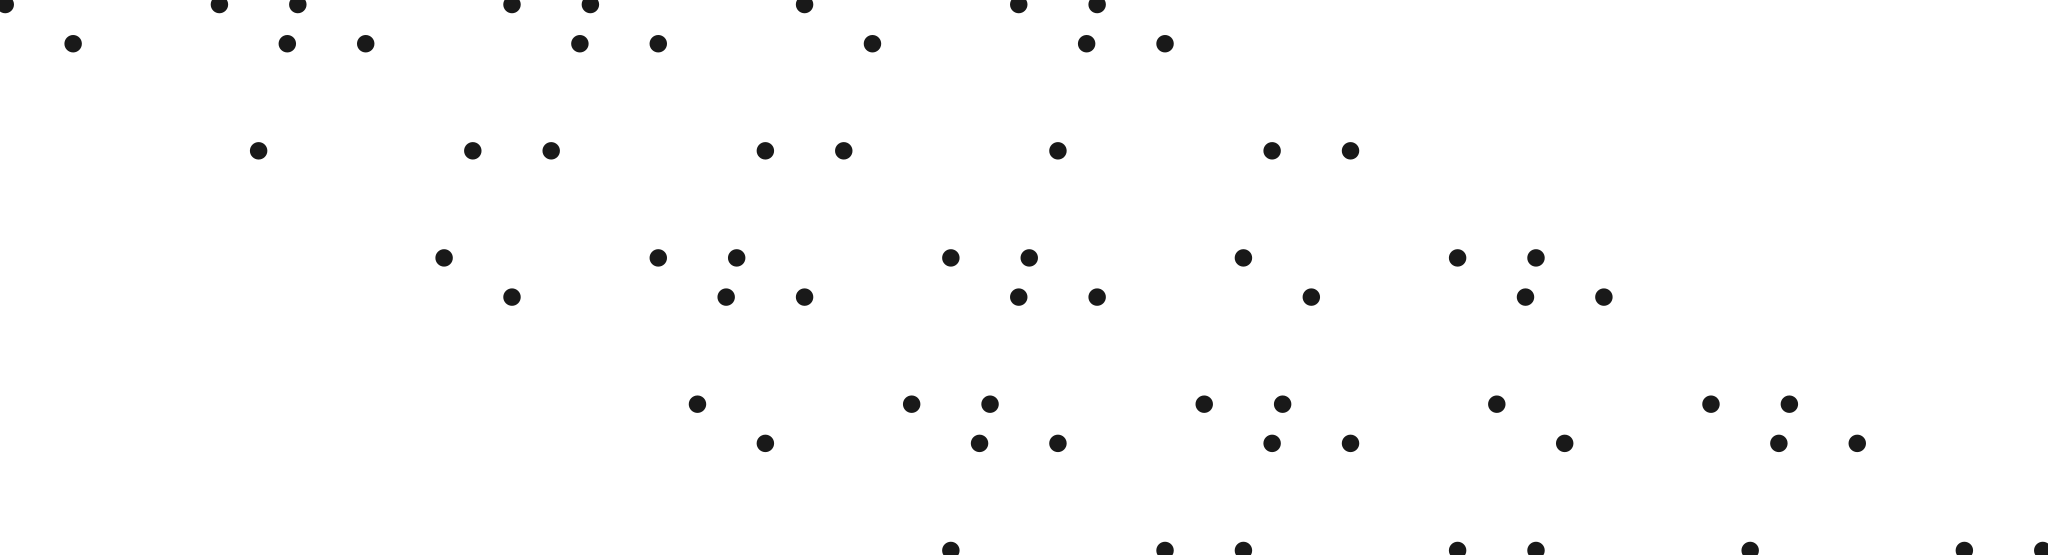
\includegraphics[width=0.3\textwidth]{finiteSectionForTileGeneration}
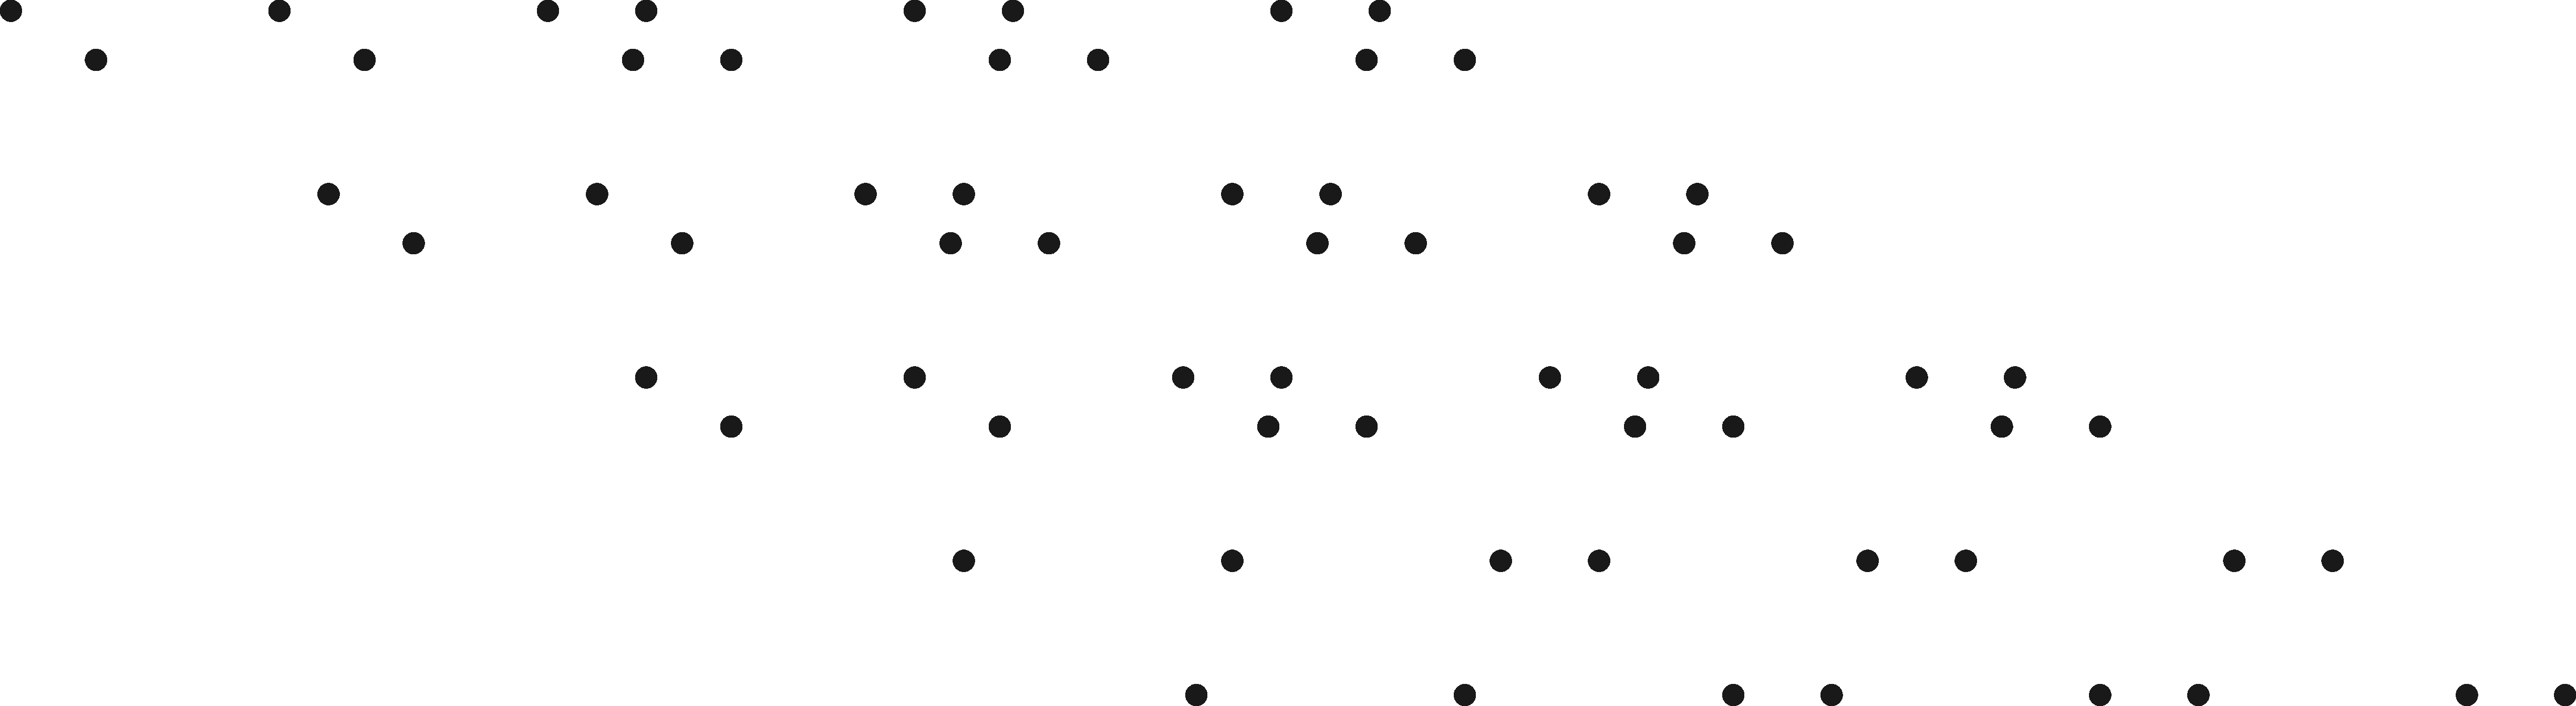
\includegraphics[width=0.3\textwidth]{finiteSectionForTileGeneration02}
\caption{Example of just $2$ finite sections.}
\label{fig:finiteSectionForTileGeneration}
\end{figure}

\begin{figure}[h]
\centering
\includegraphics[width=0.14\textwidth]{finiteSectionForTileGeneration/tile003}
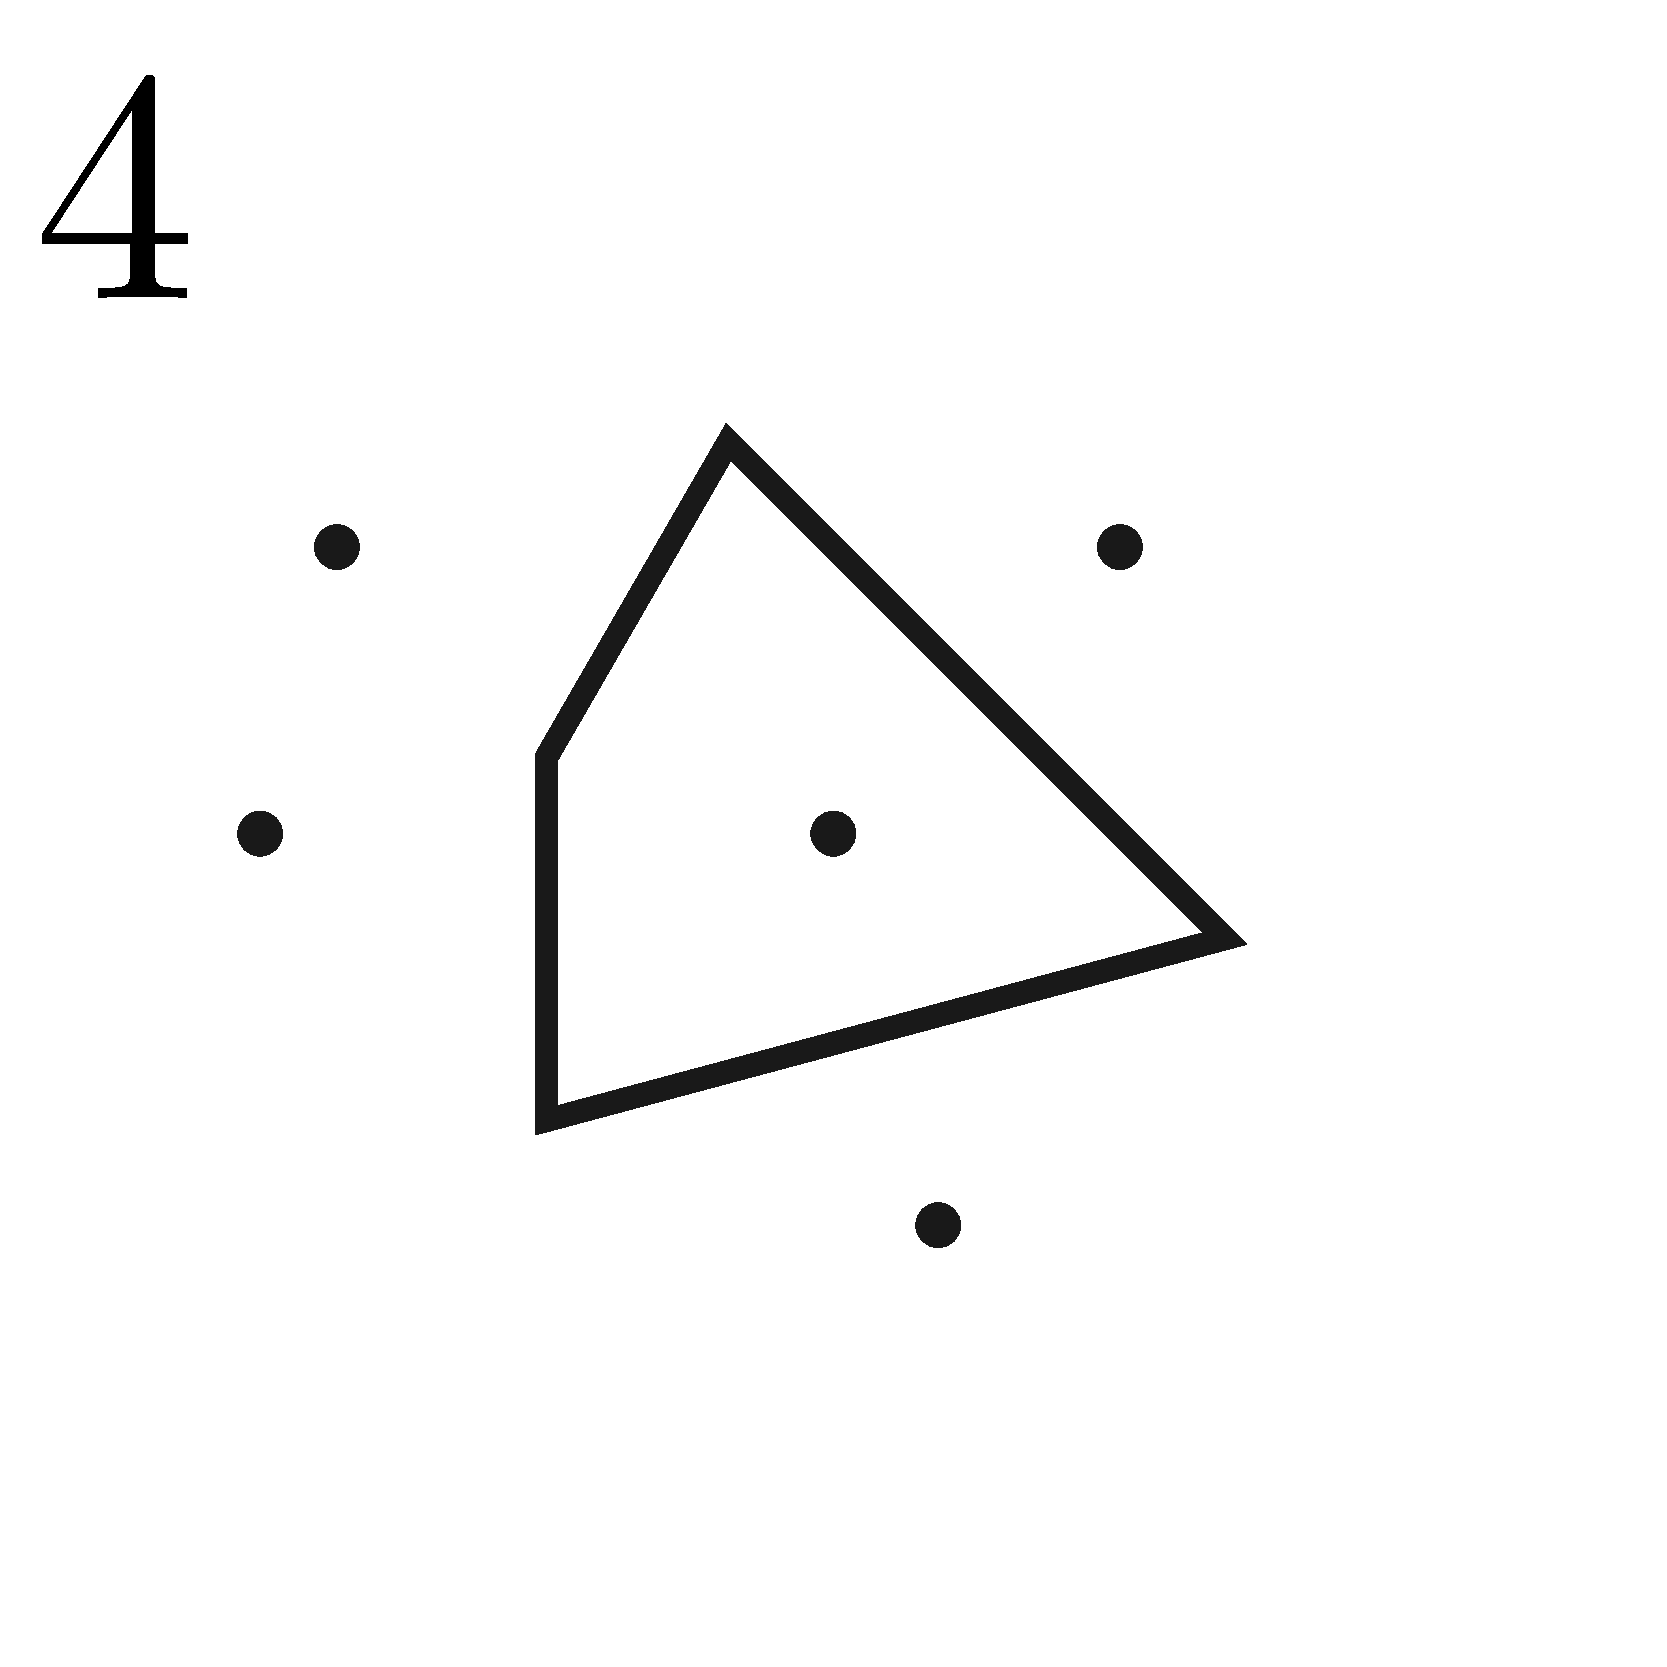
\includegraphics[width=0.14\textwidth]{finiteSectionForTileGeneration/tile004}
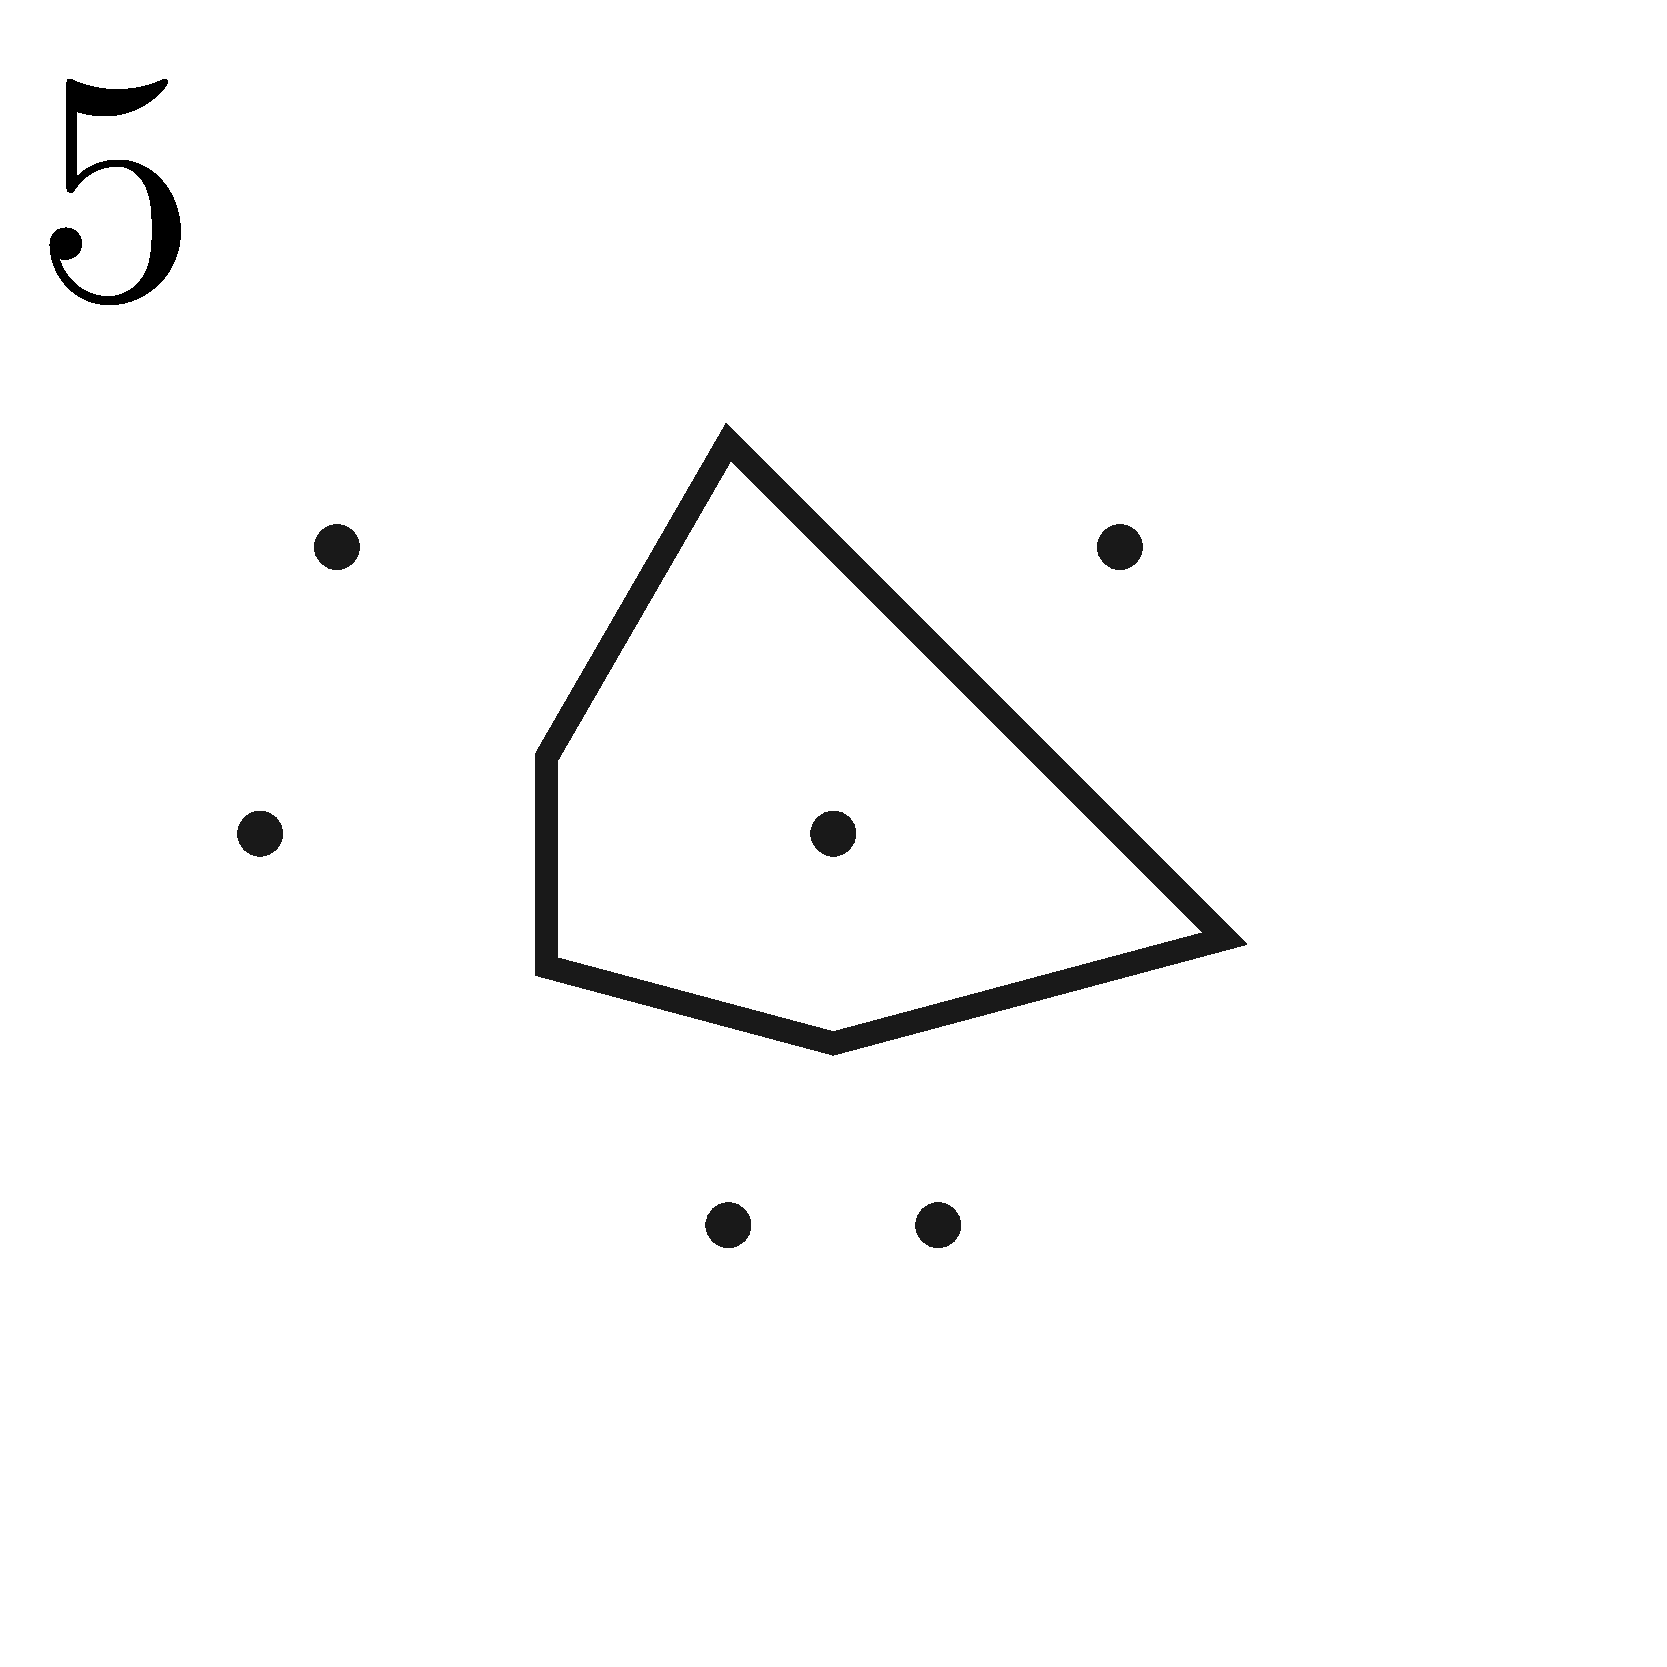
\includegraphics[width=0.14\textwidth]{finiteSectionForTileGeneration/tile005}
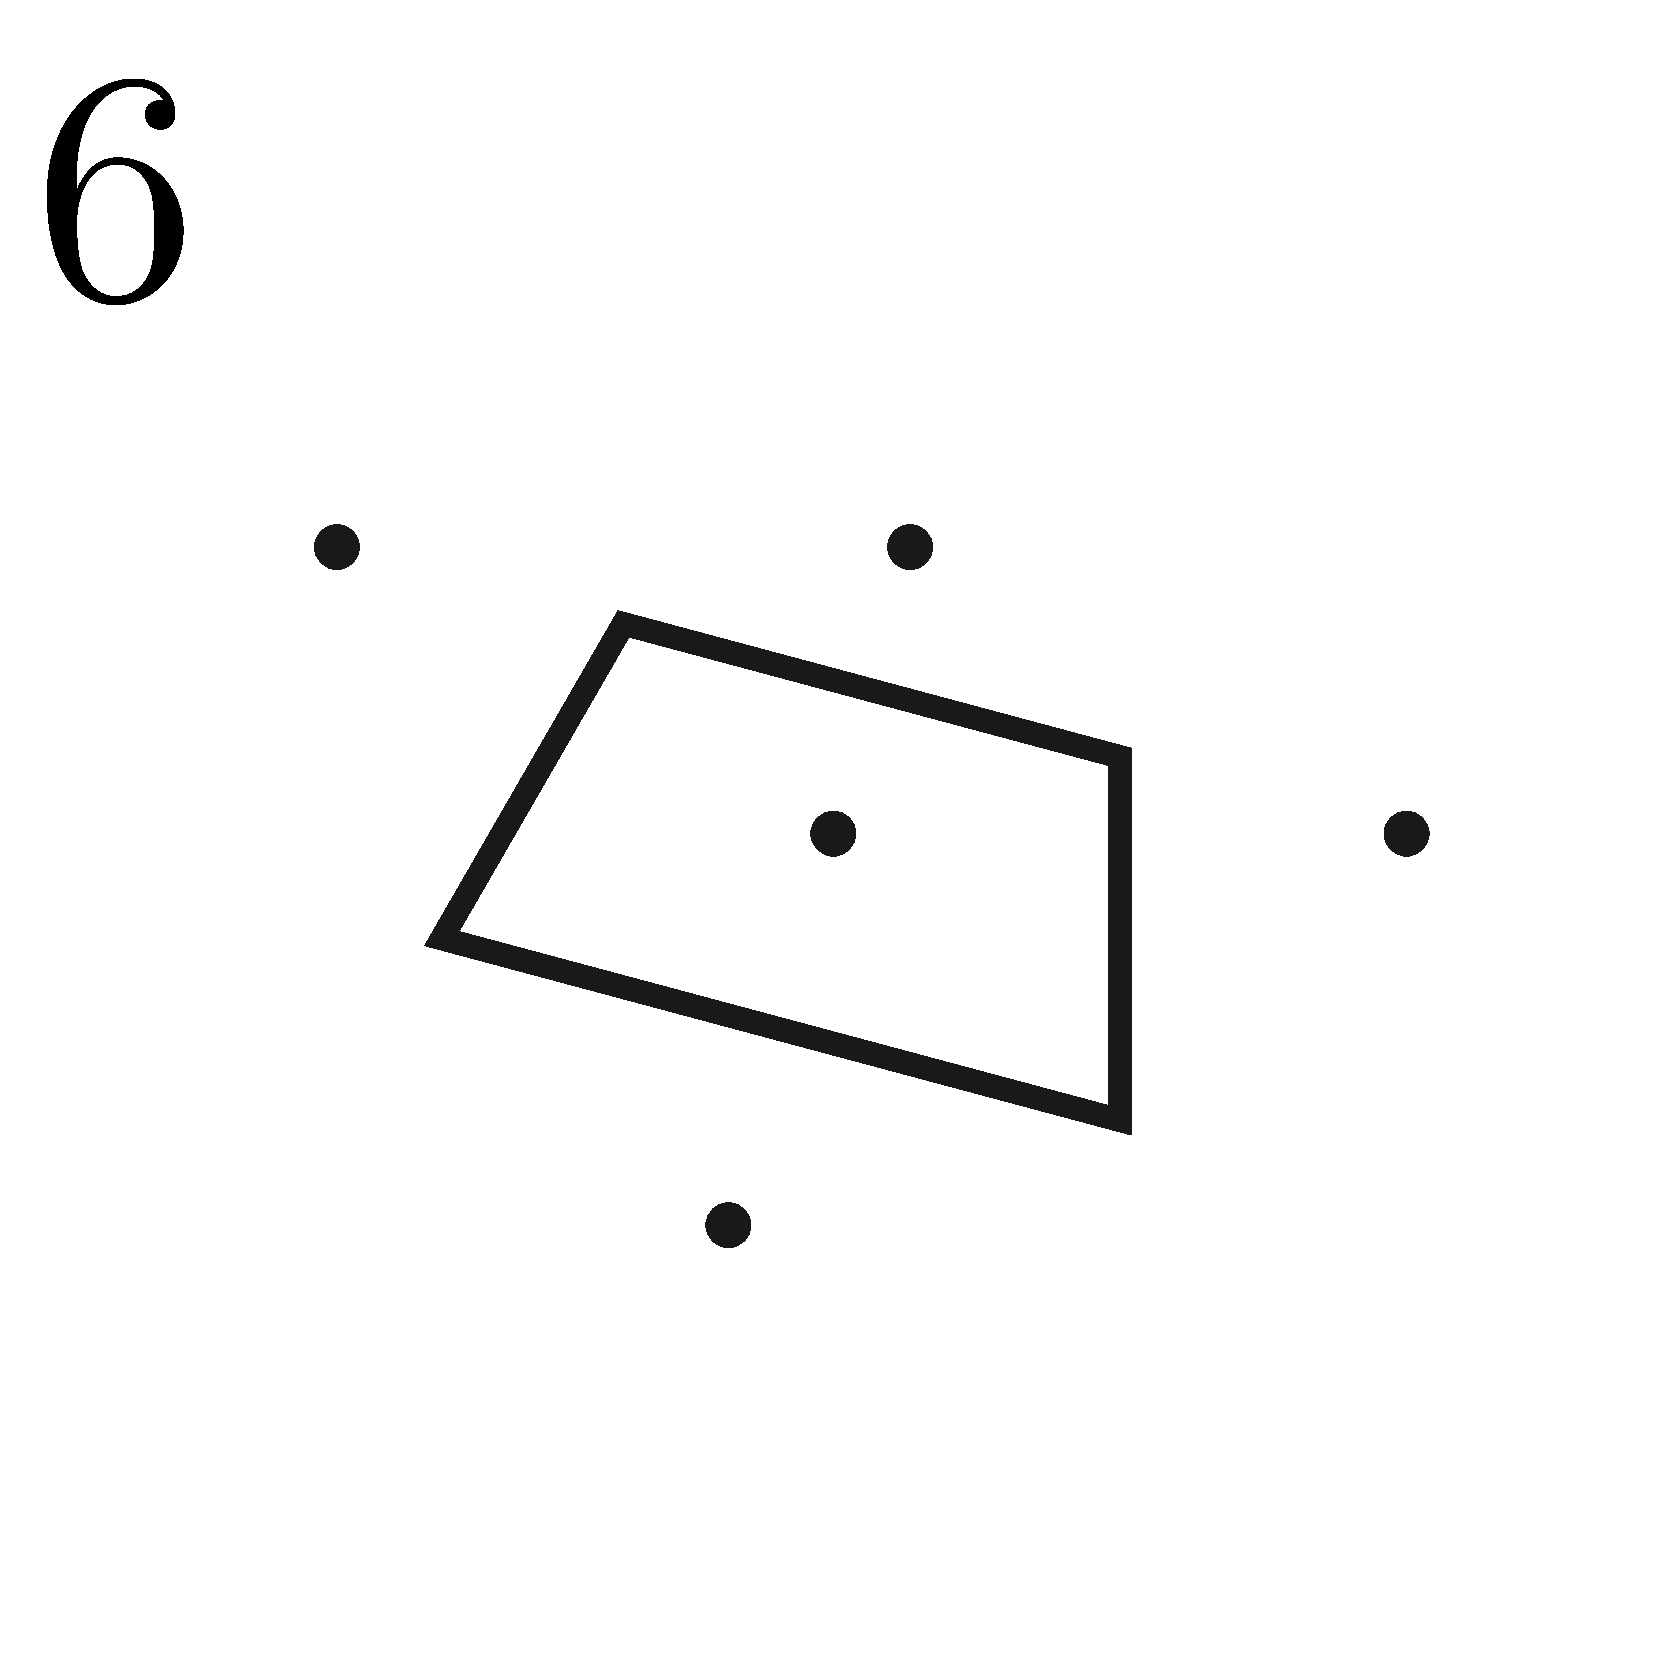
\includegraphics[width=0.14\textwidth]{finiteSectionForTileGeneration/tile006}
\caption{Example of one voronoi polygon in four different orientations.}
\label{fig:finiteSectionForTileGeneration:more}
\end{figure}

To justify that the algorithm finds all voronoi polygons for a given window consider, that the shape of each voronoi polygon is determined by the points of the quasicrystal, that are distant at most $2L\cdot\hat{R}_c$ from the center of the polygon. In other words, the shape is only determined by a finite section of the quasicrystal. Each finite section of the quasicrystal with a rhombic window is described by two finite sections of a one-dimensional quasicrystal. Each finite section of one-dimensional quasicrystal with $n+1$ points is described by a finite word of the quasicrystal, every such word is present in the language $\mathcal{L}_{\ell}(n)$.

\subsection{Determine sufficient $n$}
Part of the algorithm that was not covered in detail is how to determine the length of a word sufficient to cover a circle of radius $2L\cdot\hat{R}_c$. First a rhombus is circumscribed to the circle of the radius $2L\cdot\hat{R}_c$. The side of such rhombus is $4$ times larger than the circle radius. Then such $n$ has to be found that a finite section of one-dimensional quasicrystal corresponding to each word from $\mathcal{L}_{\ell}(n)$ has to be at least as long as the side of the circumscribed rhombus. 
There are several approaches, two are described here. 

\begin{figure}[h]
\centering
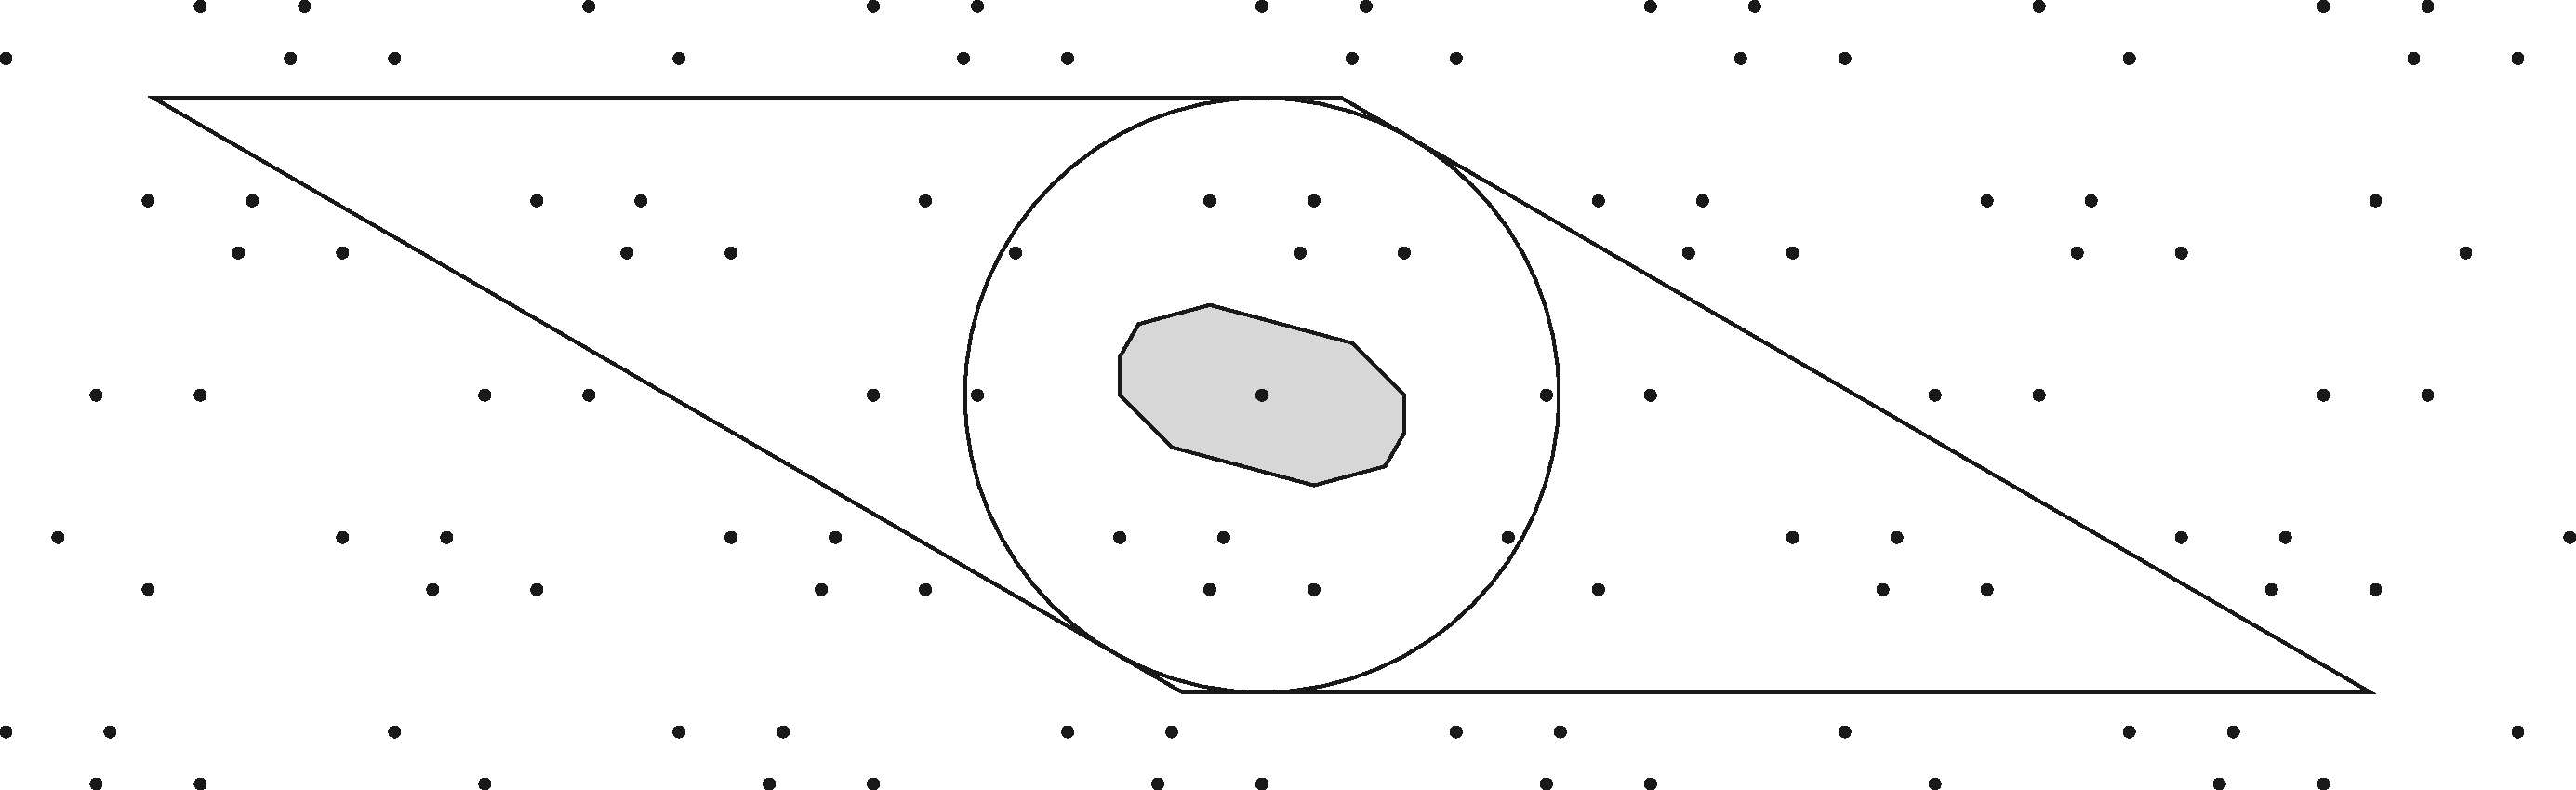
\includegraphics[width=0.9\textwidth]{wordLenghtEstimate}
\caption{Finite section of a quasicrystal containing the origin. The circle has a radius $2L\cdot\hat{R}_c$ and contains all the points of the quasicrystal that determine the shape of the voronoi polygon for the origin. The circumscribed rhombus contains a superset.}
\label{fig:wordLenghtEstimate}
\end{figure}

One way is to get the smallest distance $S$ for the one-dimensional quasicrystal and set $n = \left\lceil\frac{8L\cdot\hat{R}_c}{S}\right\rceil$. 

The second way is to start with $n=2$, test each word of the language $\mathcal{L}_{\ell}(n)$ and increase by $1$ until $n$ is sufficient. 

The second way takes more time to compute but produces better estimate, which will be desirable once analyzing quasicrystals with a general window.

\subsection{Different orientations}
As is apparent from Figure \ref{fig:finiteSectionForTileGeneration:more}, the same shape of a voronoi polygon appears in the quasicrystal in more orientations. This section covers the analysis of different orientations of voronoi polygons. 

It is helpful to see the connection between the domain of the voronoi polygon and it's $\ast$ image in the window of the quasicrystal. Figure \ref{fig:windowWithDomain} shows a voronoi polygon from the quasicrystal with the window size $2-7\beta$, the window and $\ast$ image of it's domain and it's center. 

\begin{figure}[h]
\centering
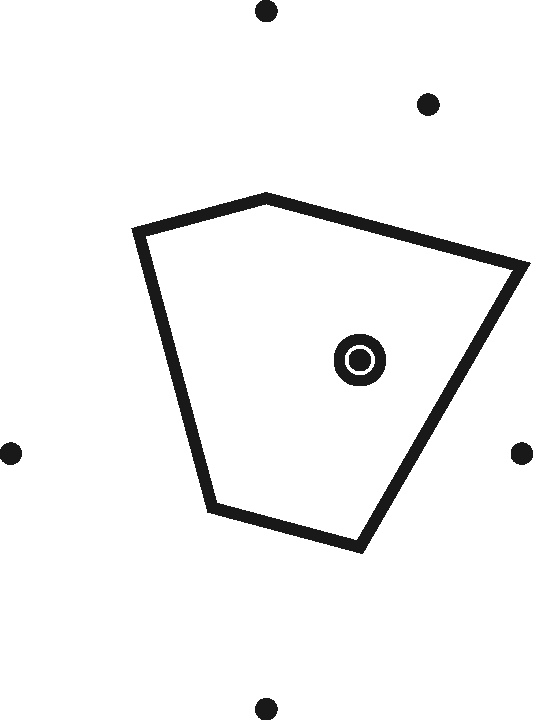
\includegraphics[width=0.12\textwidth]{catalogRhombusSingle/tileForDomain}
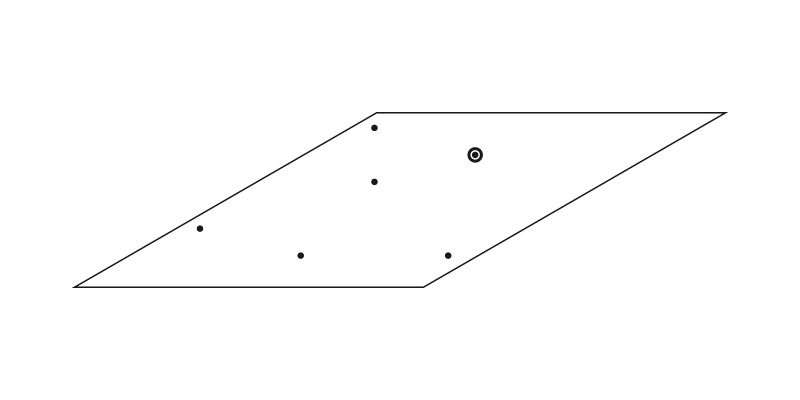
\includegraphics[width=0.55\textwidth]{catalogRhombusSingle/windowWithDomain}
\caption{A voronoi polygon with it's center and domain and the $\ast$ image in the window of the quasicrystal.}
\label{fig:windowWithDomain}
\end{figure}

It is clear that a voronoi polygon can appear in a quasicrystal only if the $\ast$ image of it's domain and center fits inside the window. Therefore a section of the window can be associated with a voronoi polygon through it's center. The section shows where in the window the $\ast$ image of the center can be so that the $\ast$ image of the domain fits in also (Figure \ref{fig:windowWithSection}). 

\begin{figure}[h]
\centering
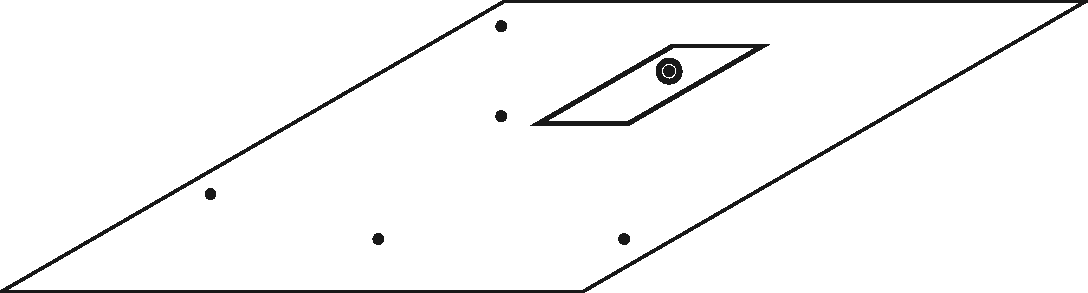
\includegraphics[width=0.55\textwidth]{catalogRhombusSingle/windowWithSection}
\caption{A window with the $\ast$ image of the domain and the center from the Figure \ref{fig:windowWithDomain} with the associated section.}
\label{fig:windowWithSection}
\end{figure}

In fact the entire window can be divided in such sections. Every point of the quasicrystal whose $\ast$ image falls within one section is the center of a voronoi polygon of the same shape (Figure \ref{fig:windowWithDivision}). The algorithm for producing such division will be covered in the next section.  

\begin{figure}[h]
\centering
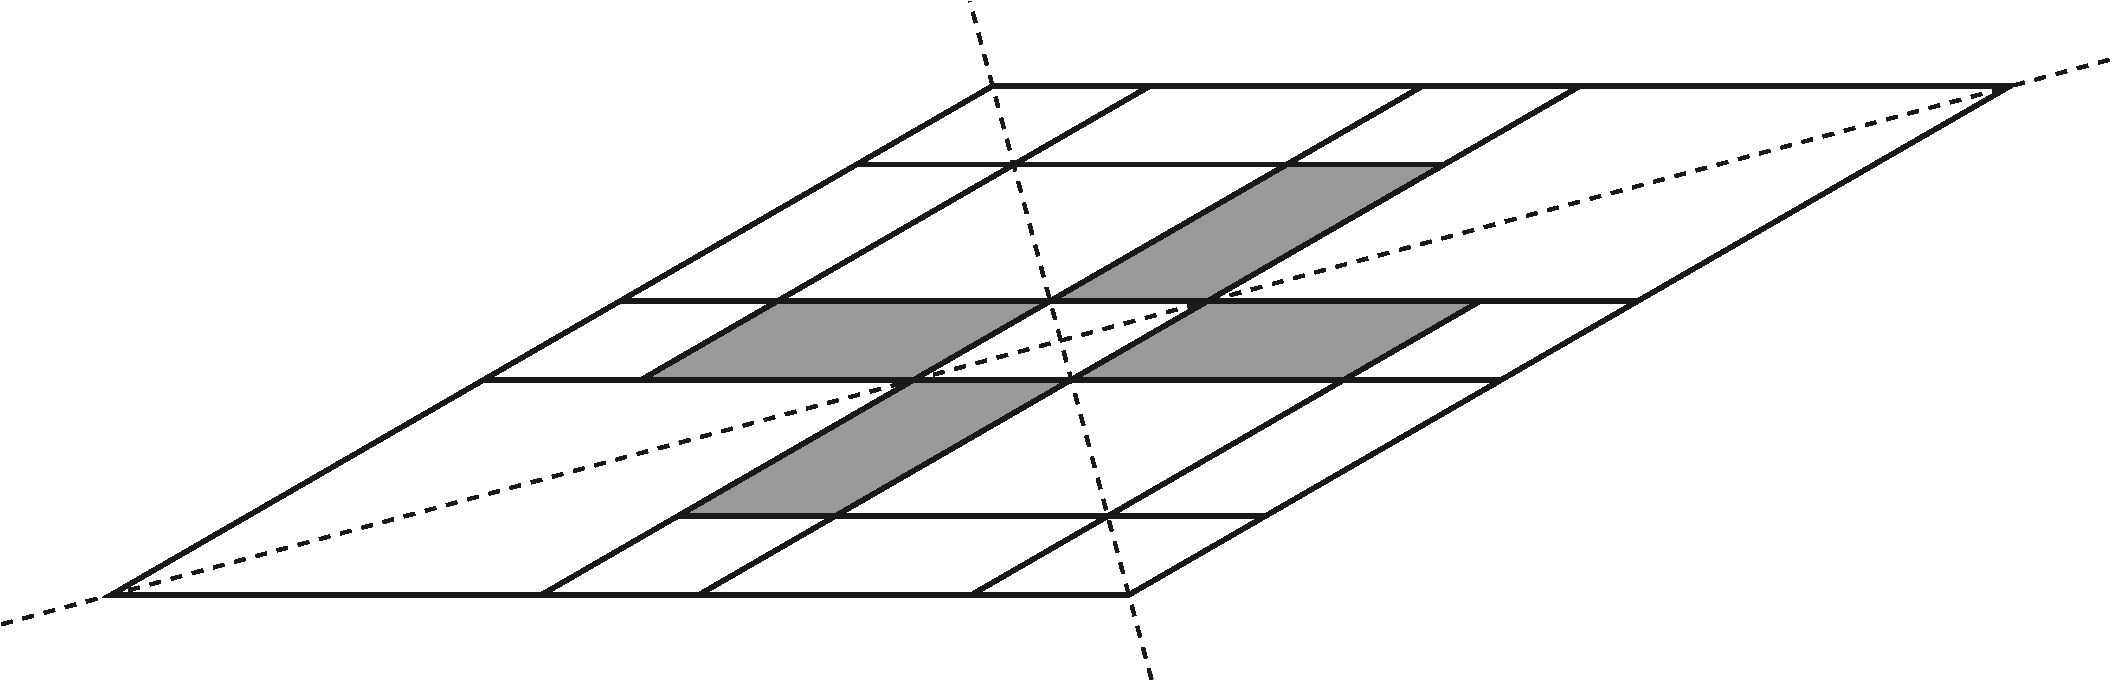
\includegraphics[width=0.606\textwidth]{catalogRhombusSingle/windowWithDivision}
\caption{A window with the division into sections by the shape of corresponding voronoi polygon.}
\label{fig:windowWithDivision}
\end{figure}

From the division two axis of symmetry are apparent. These are the sources of the different orientations of the voronoi polygons of the same shape. The highlighted sections in the Figure \ref{fig:windowWithDivision} correspond to the four voronoi polygons form the Figure \ref{fig:finiteSectionForTileGeneration:more}

\subsection{Dividing a rhombic window into sections by the shape of the corresponding voronoi polygon}
Algorithm for checking whether a set of points belongs to the quasicrystal also produces the shape of the section of the window. 

Let $\Omega$ be a rhombic window, $V$ one of the voronoi polygons in the quasicrystal $\quasi{\Omega}$, $c\in M$ the center of $V$, $D = \{p_1,\dots,p_k\}\subset M$ the domain of $V$ and $q_i = p_i - c$, $i\in\hat{k}$.
Then the $\ast$ image of the center and the domain fit inside the window:
$$c^\ast\in\Omega \quad\wedge\quad c^\ast + q_i^\ast\in\Omega \quad(\forall i\in\hat{k})$$
which is equivalent to whether the image of the center $c^\ast$ fits inside translated windows:
$$c^\ast\in\Omega \quad\wedge\quad c^\ast\in\Omega-q_i^\ast \quad(\forall i\in\hat{k})$$
$$c^\ast\in\bigcap\limits_{i\in\hat{k}}(\Omega-q_i^\ast)\cap\Omega$$
Now first if the intersection is not empty then the polygon $V$ appears in the quasicrystal $\quasi{\Omega}$, this finding will be useful while analyzing quasicrystals with a general window. Also the intersection shows exactly the desired section of the window. Only if the image of the center fits inside this intersection does the image of the domain fit inside the window and that determines the shape of the voronoi polygon. 

There is however a slight caveat. The intersection might be larger than the desired section. Consider this example, in the so far analyzed quasicrystal with the window size $2\beta-7$ there is a polygon very similar in shape to the one in the Figure \ref{fig:finiteSectionForTileGeneration:more} (Figure \ref{fig:finiteSectionForTileGeneration:bigger}).
\begin{figure}[h]
\centering
\includegraphics[width=0.14\textwidth]{finiteSectionForTileGeneration/tile003}
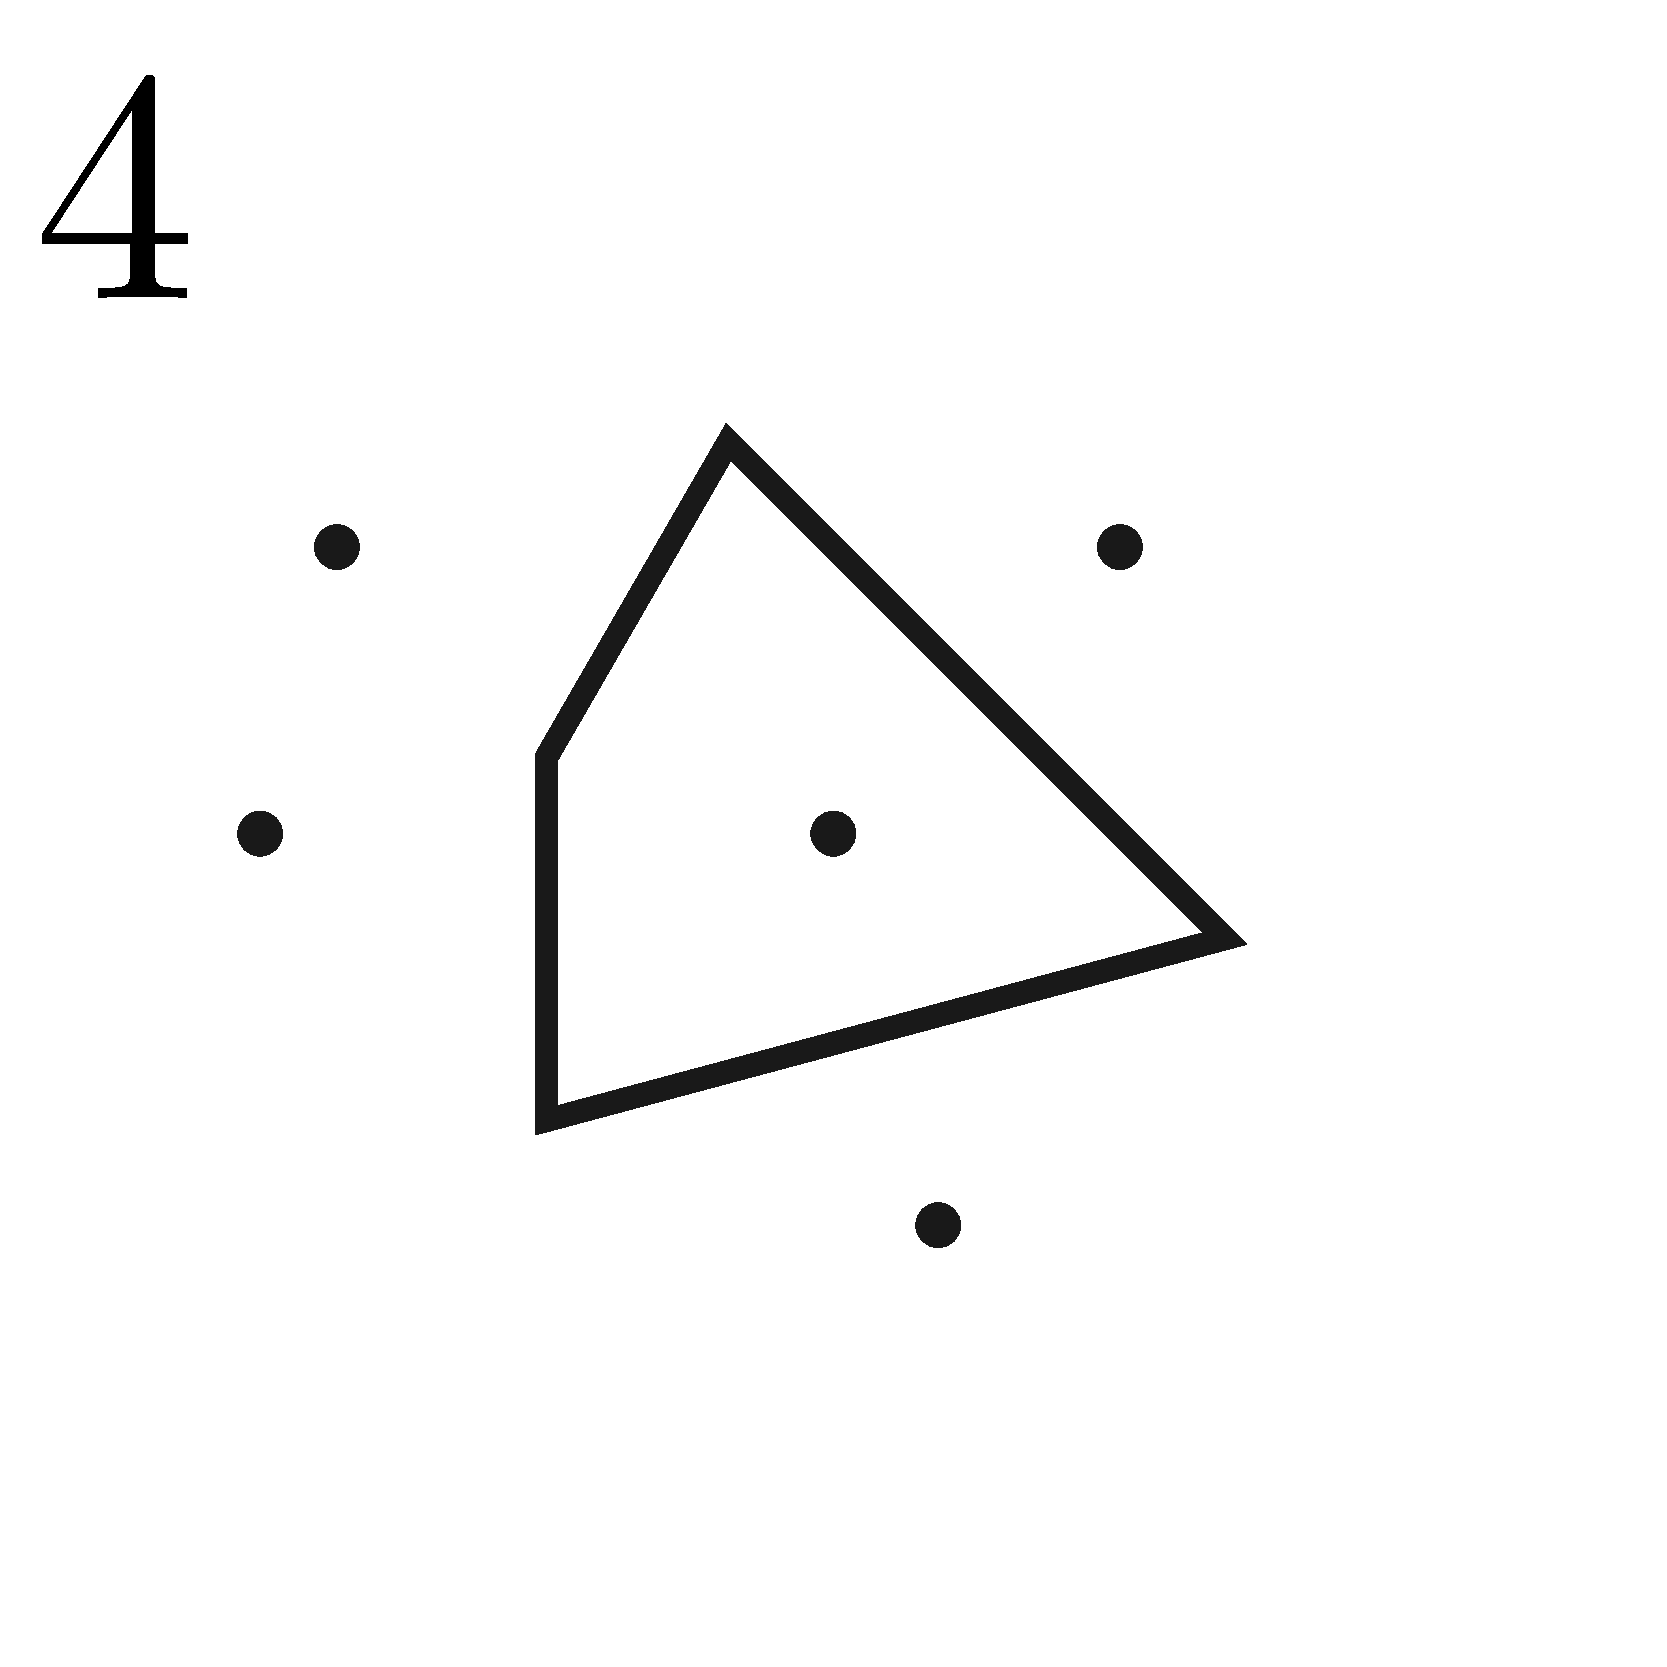
\includegraphics[width=0.14\textwidth]{finiteSectionForTileGeneration/tile004}
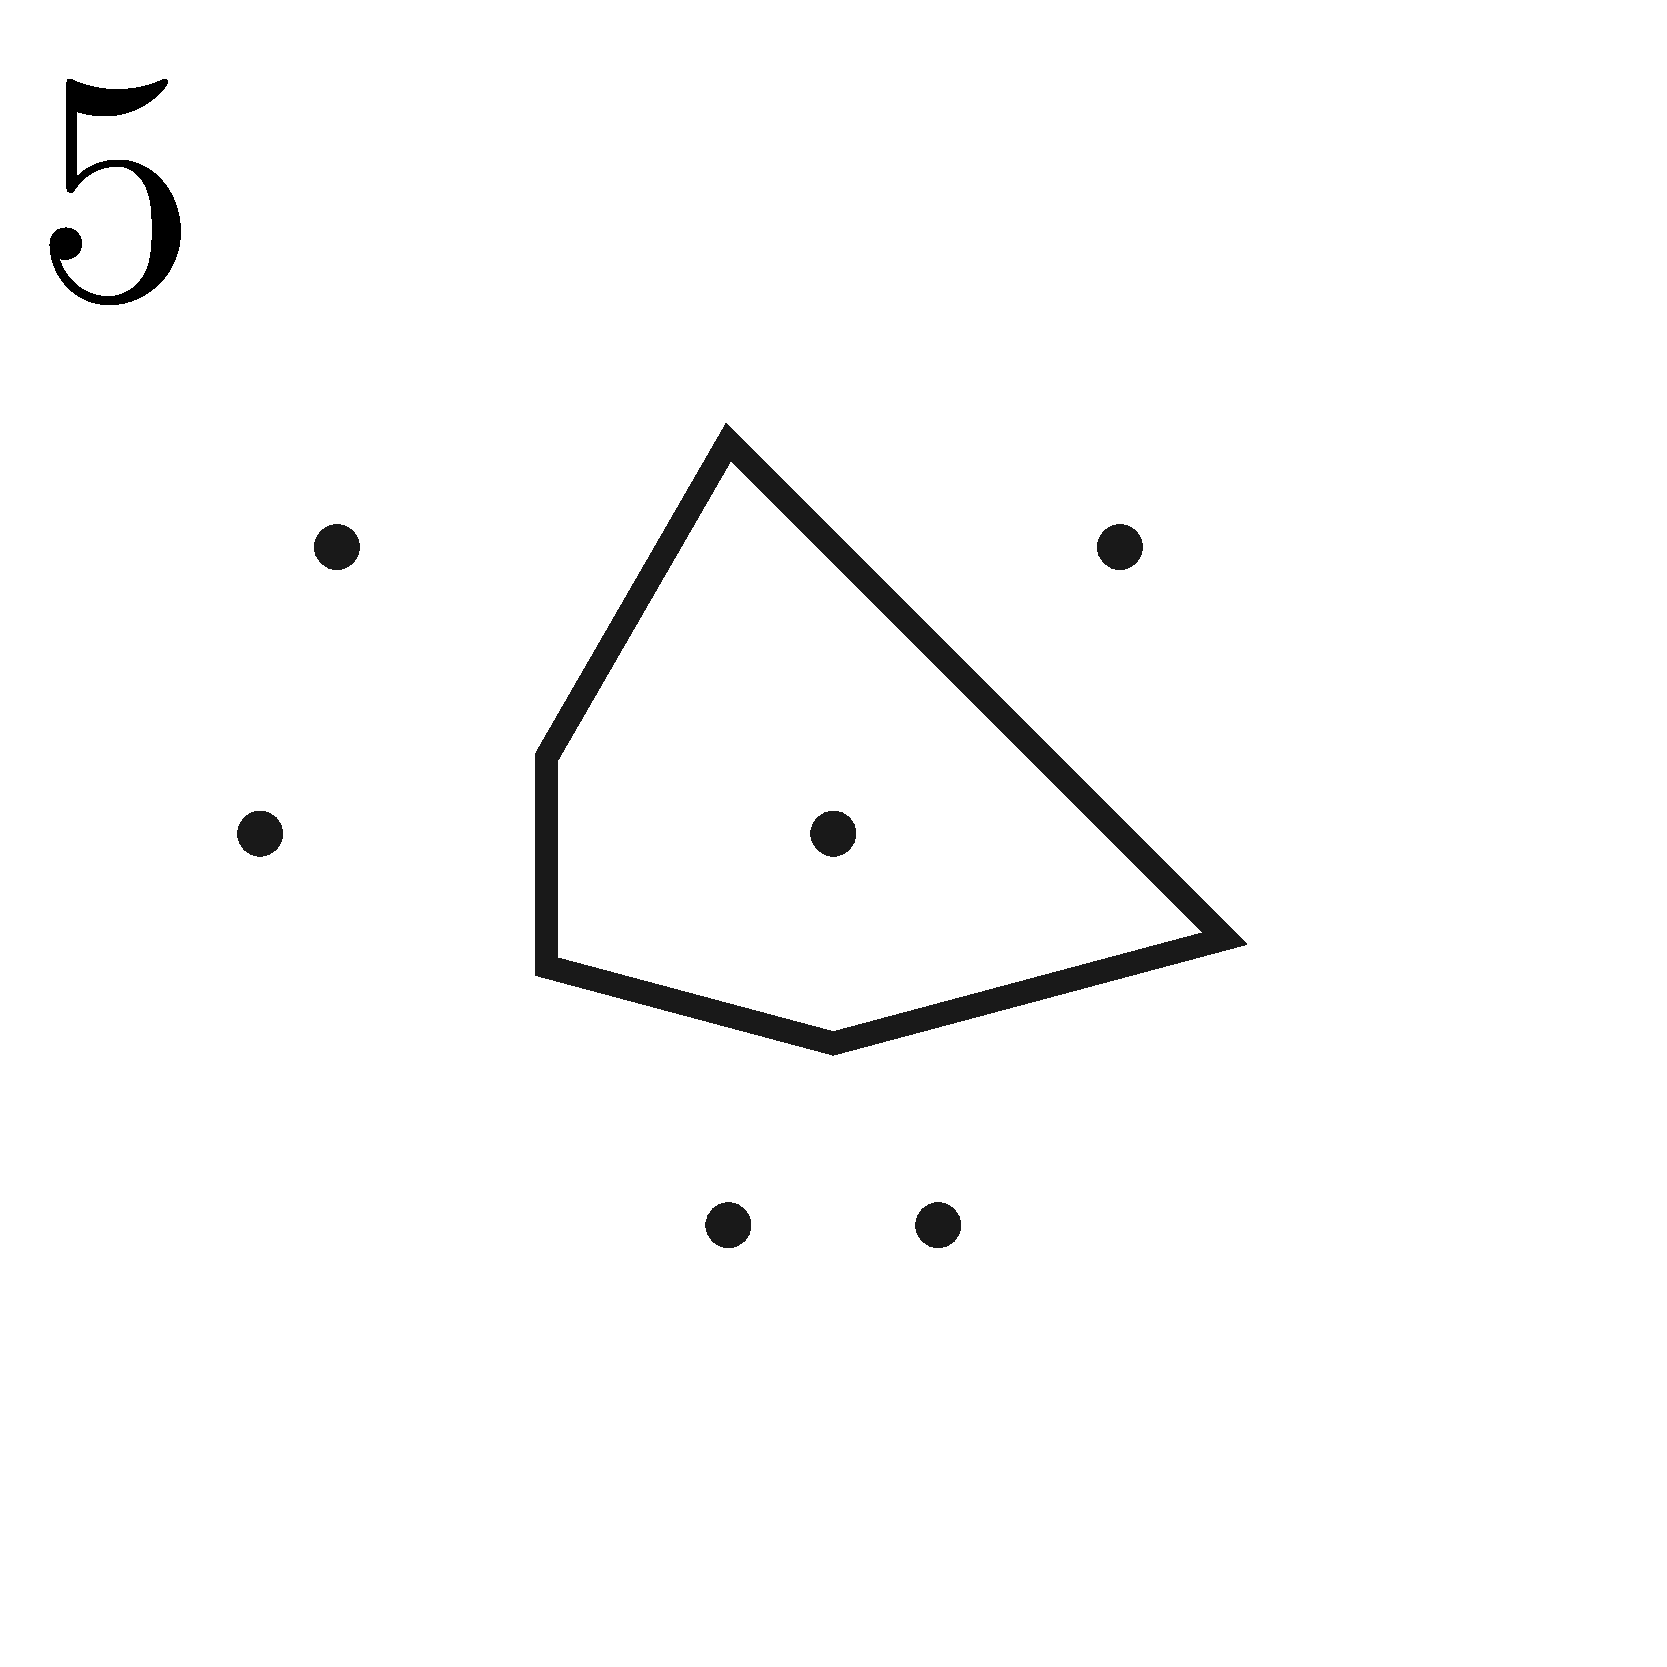
\includegraphics[width=0.14\textwidth]{finiteSectionForTileGeneration/tile005}
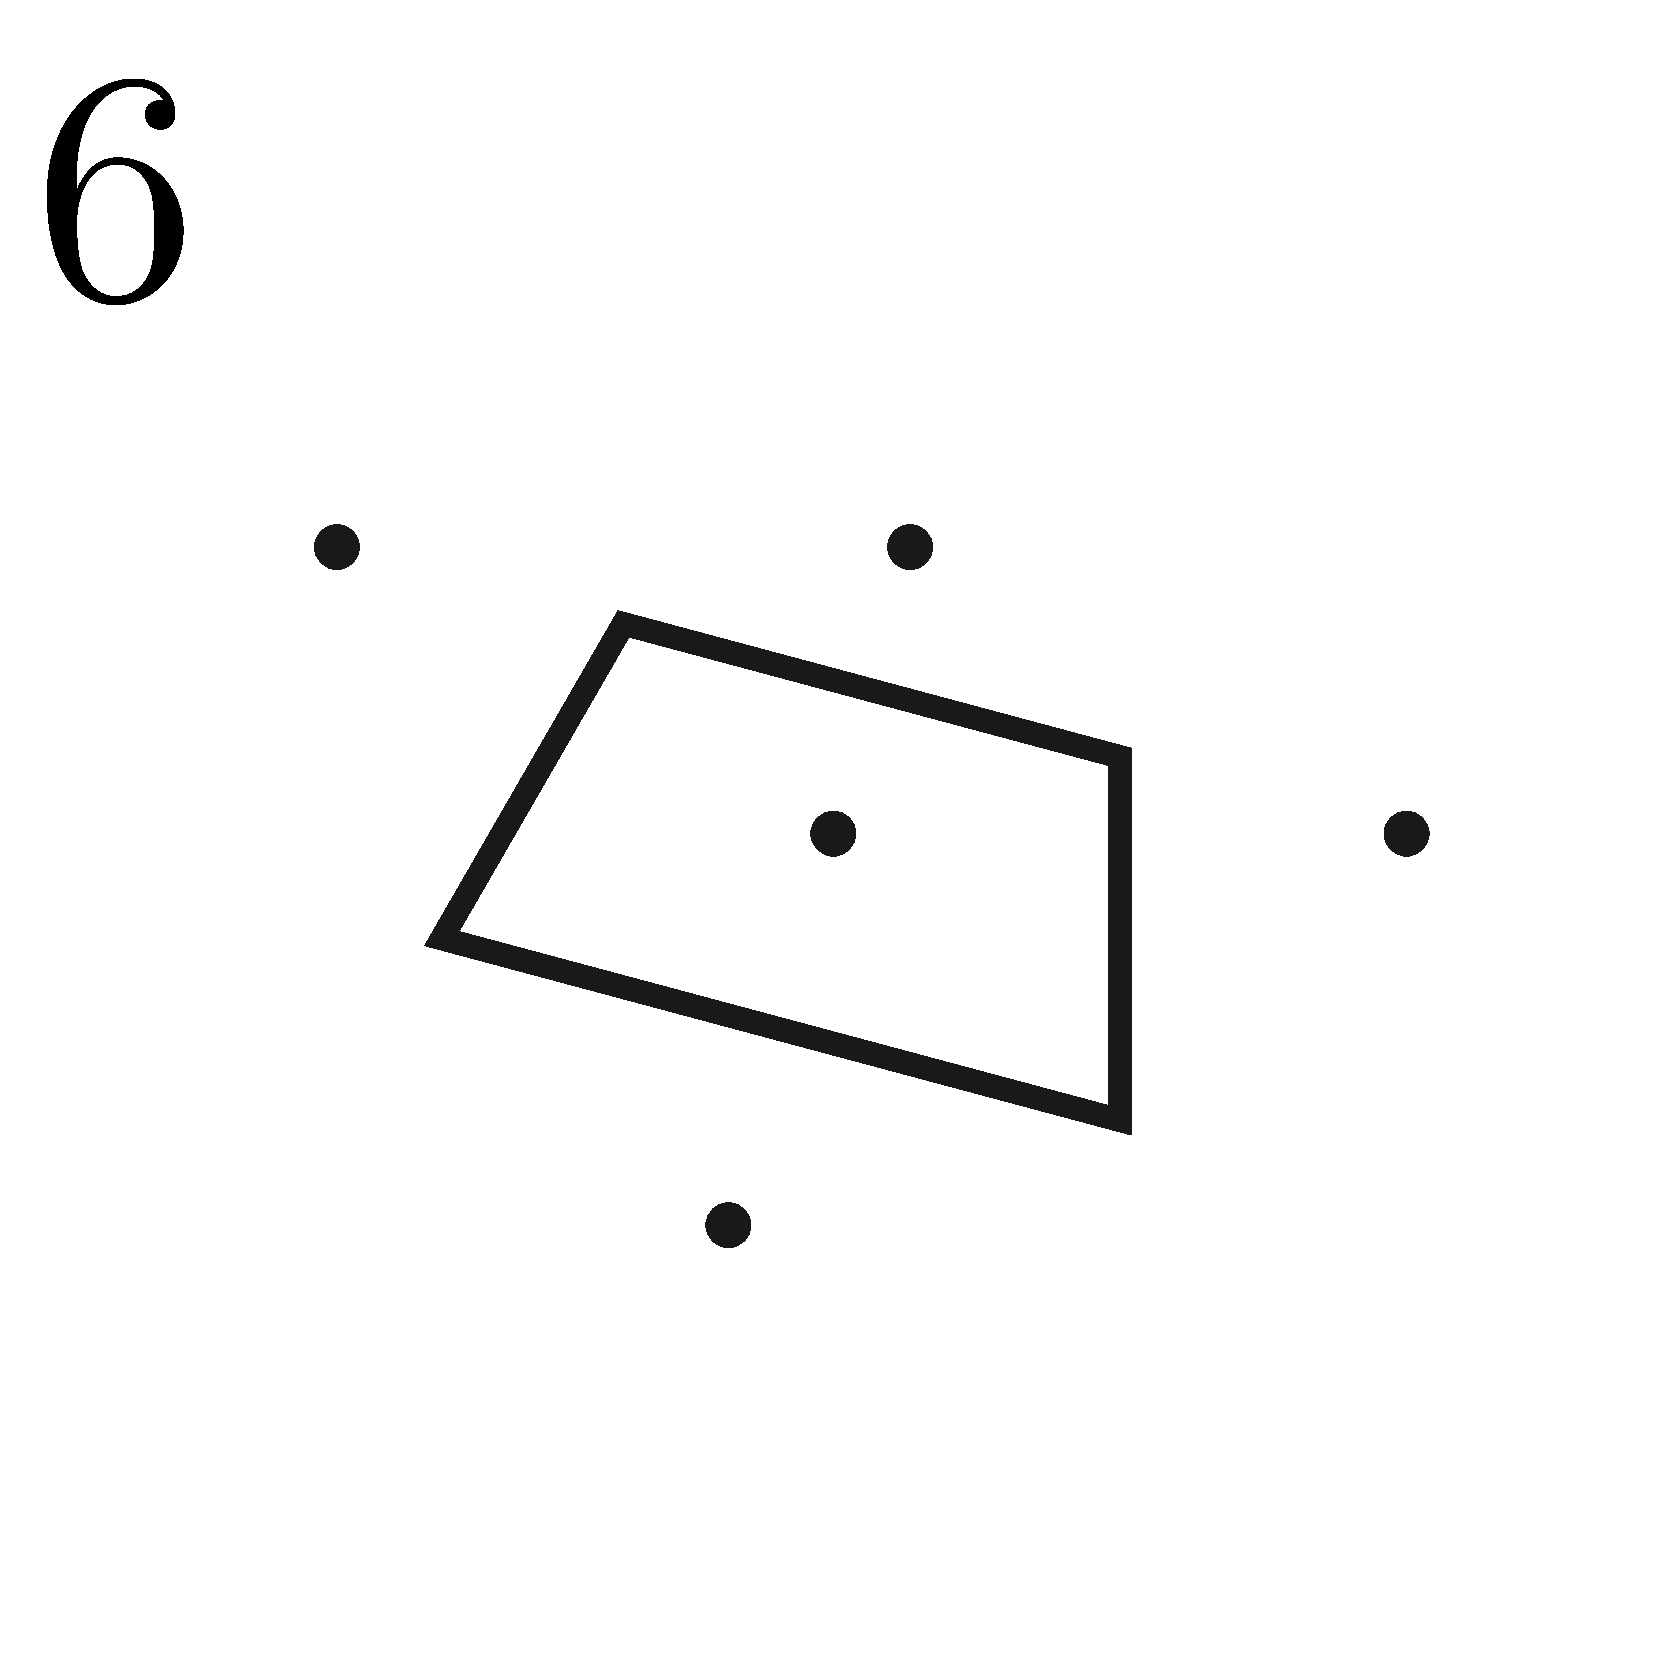
\includegraphics[width=0.14\textwidth]{finiteSectionForTileGeneration/tile006}

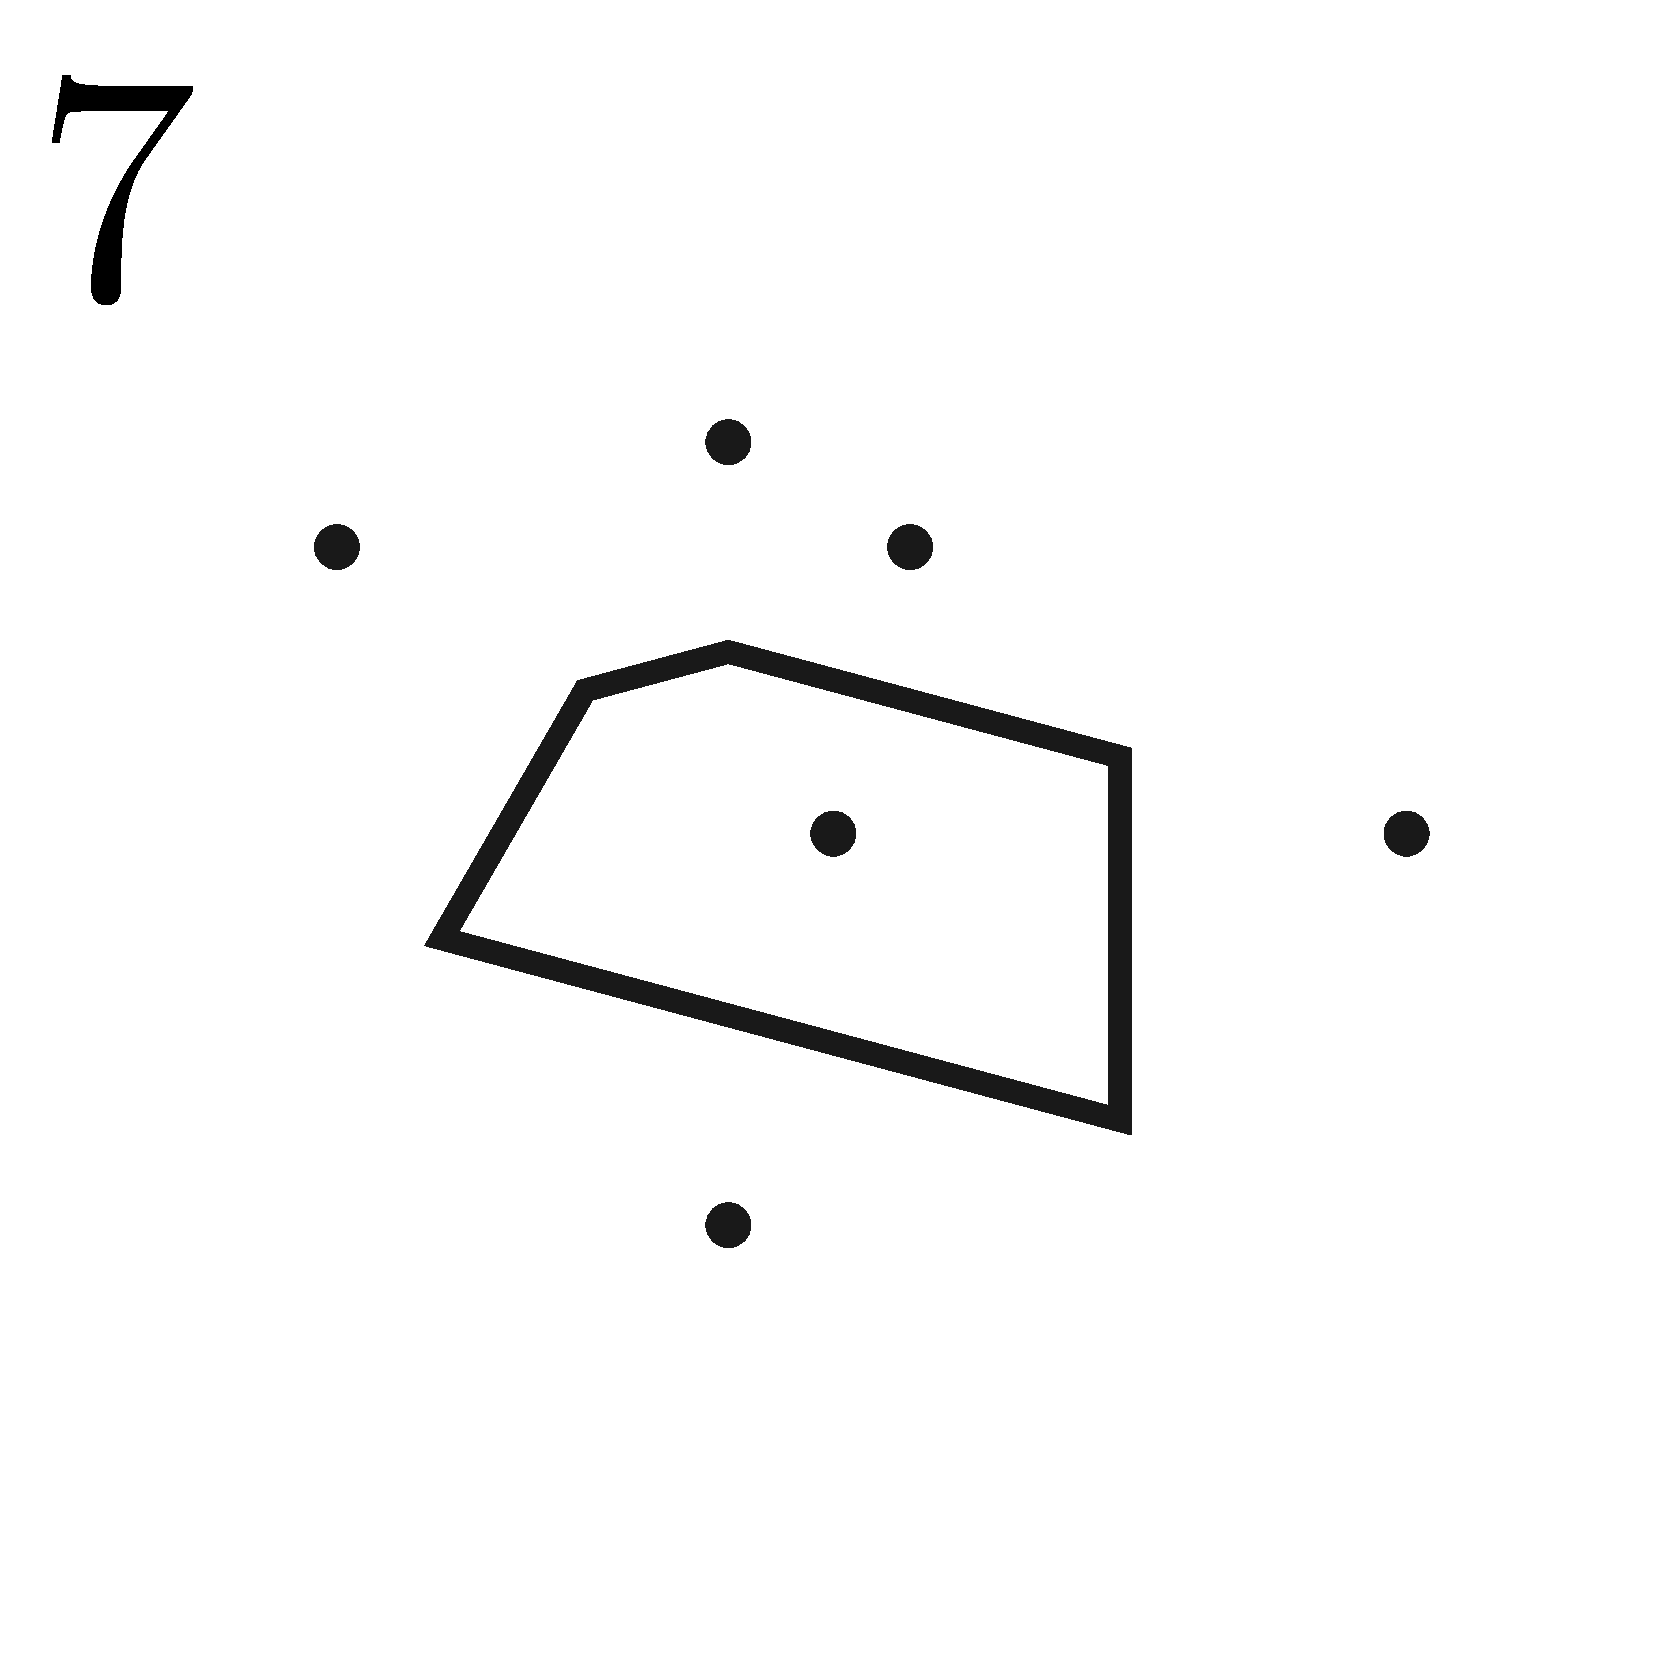
\includegraphics[width=0.14\textwidth]{finiteSectionForTileGeneration/tile007}
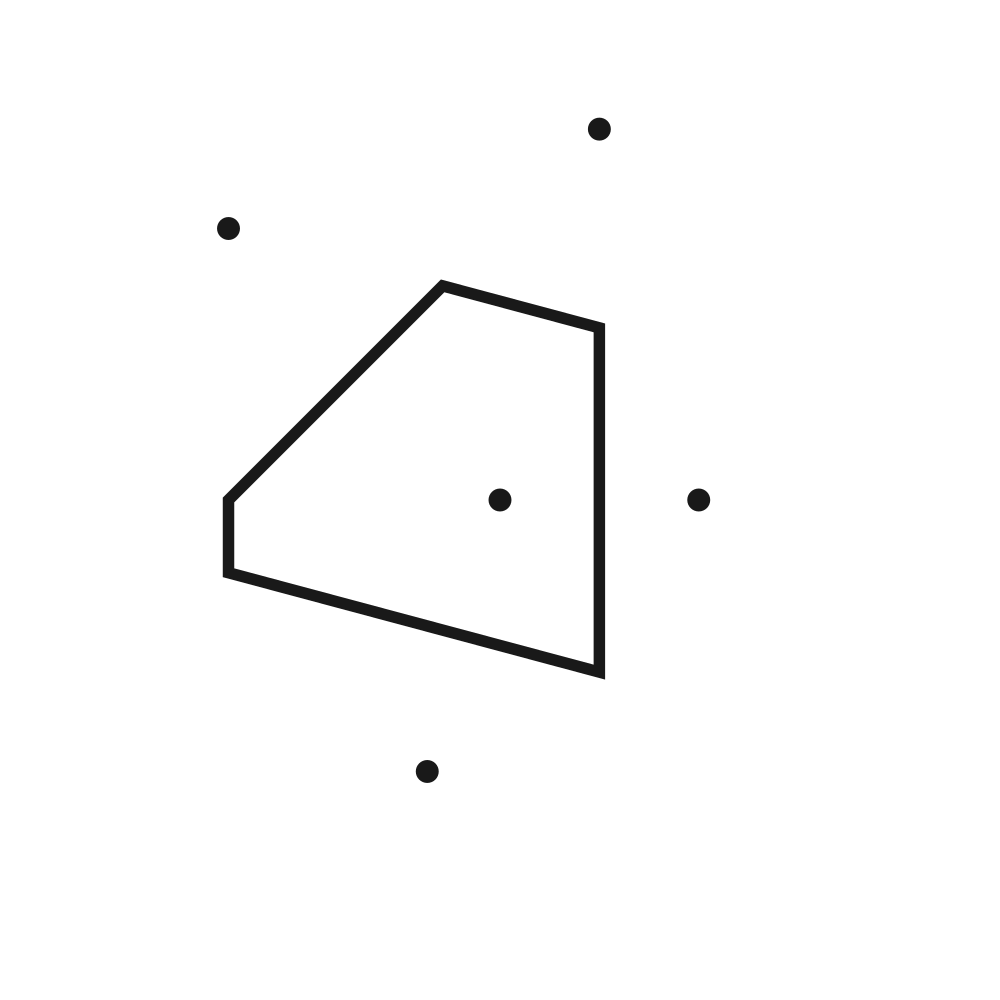
\includegraphics[width=0.14\textwidth]{finiteSectionForTileGeneration/tile008}
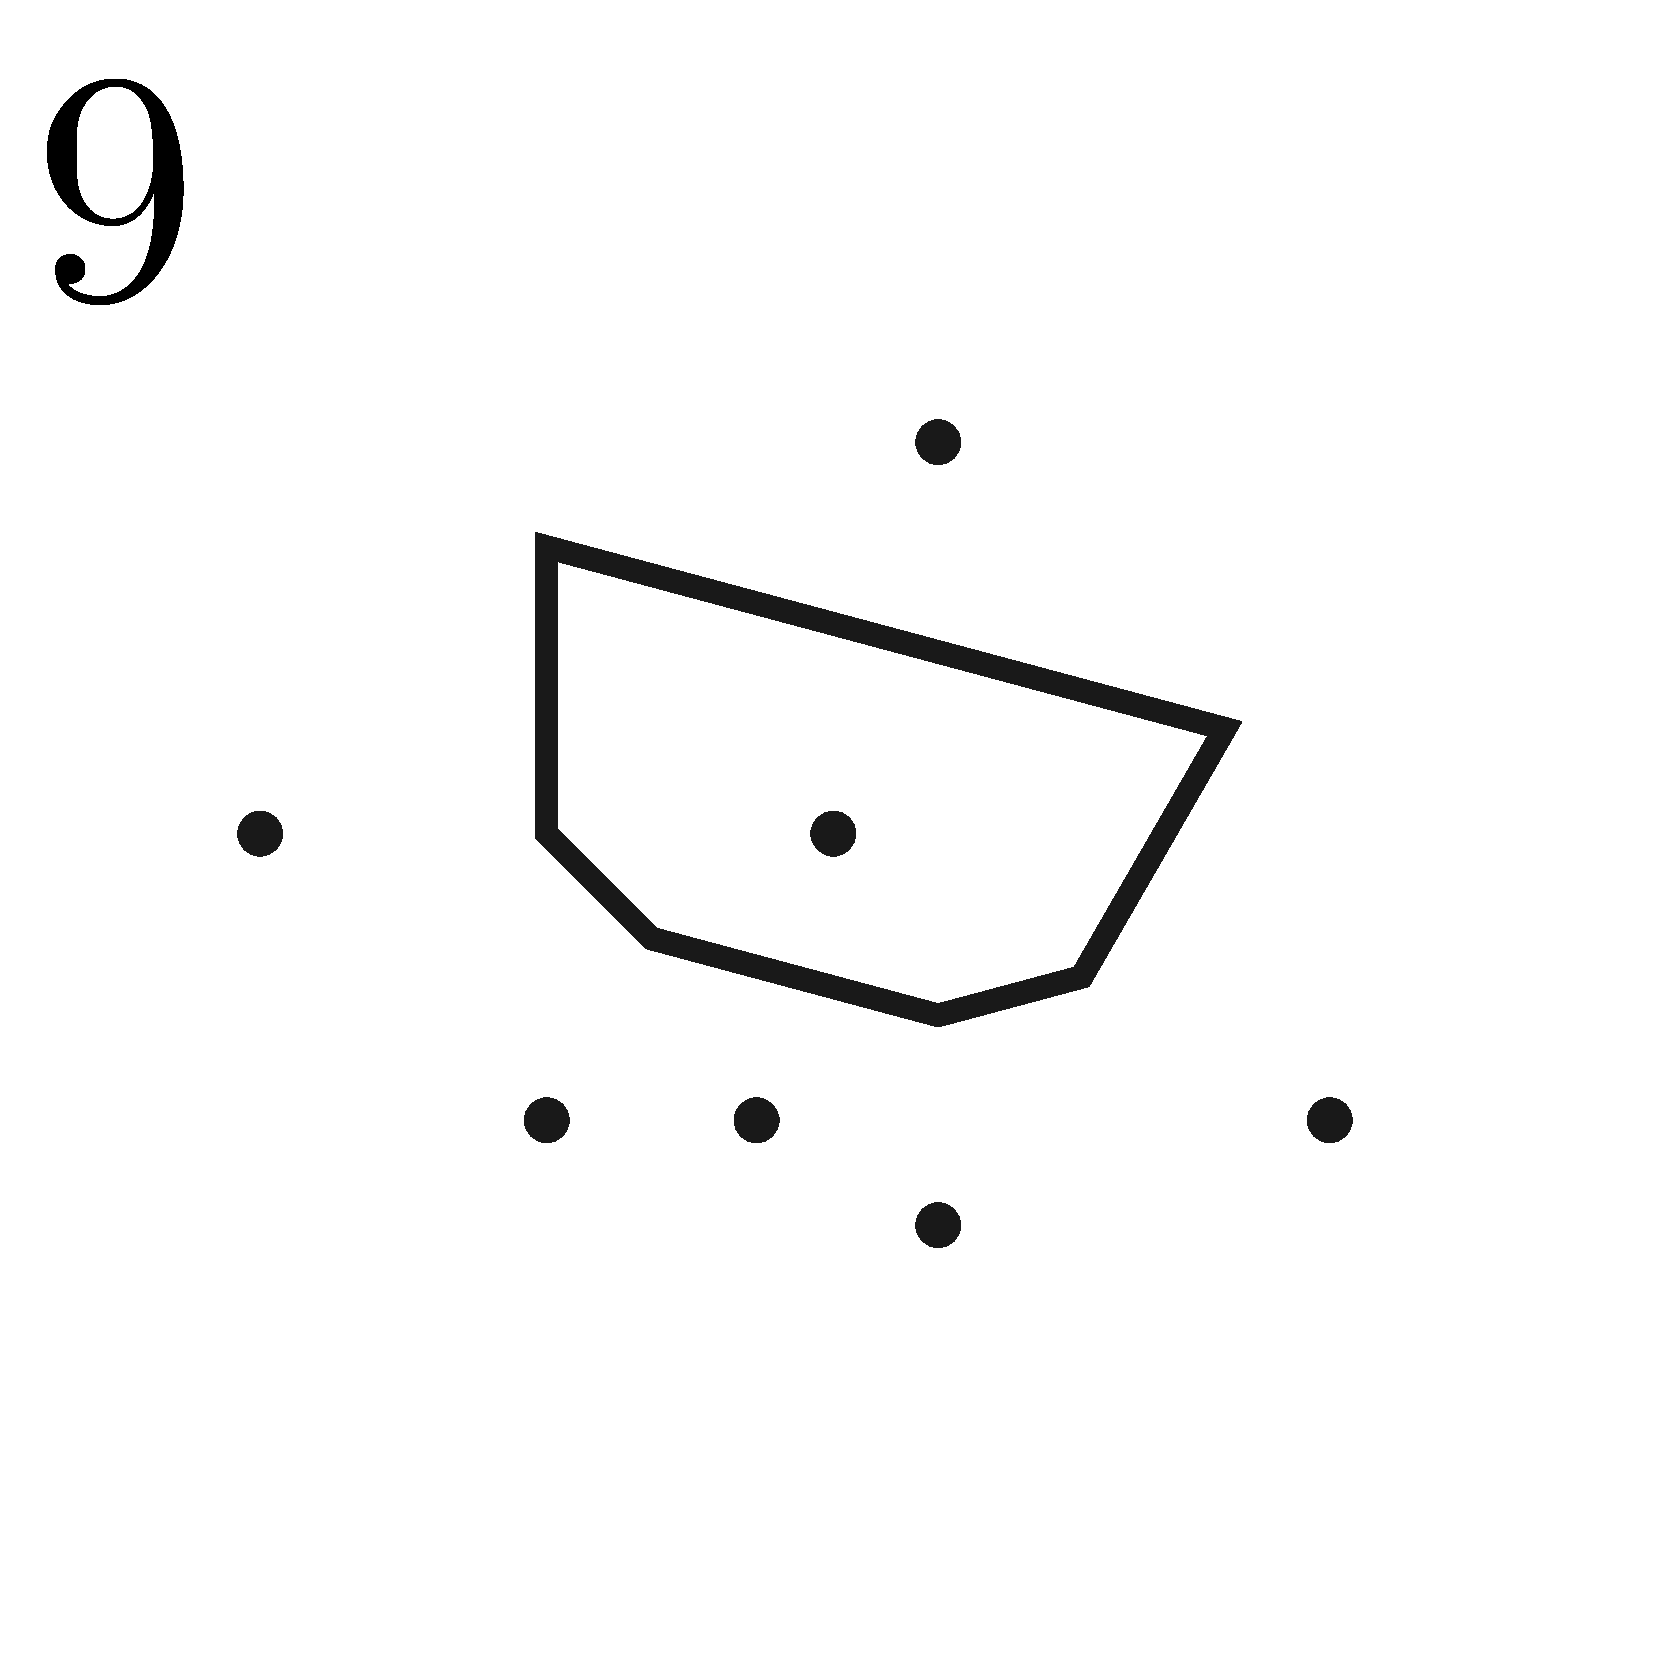
\includegraphics[width=0.14\textwidth]{finiteSectionForTileGeneration/tile009}
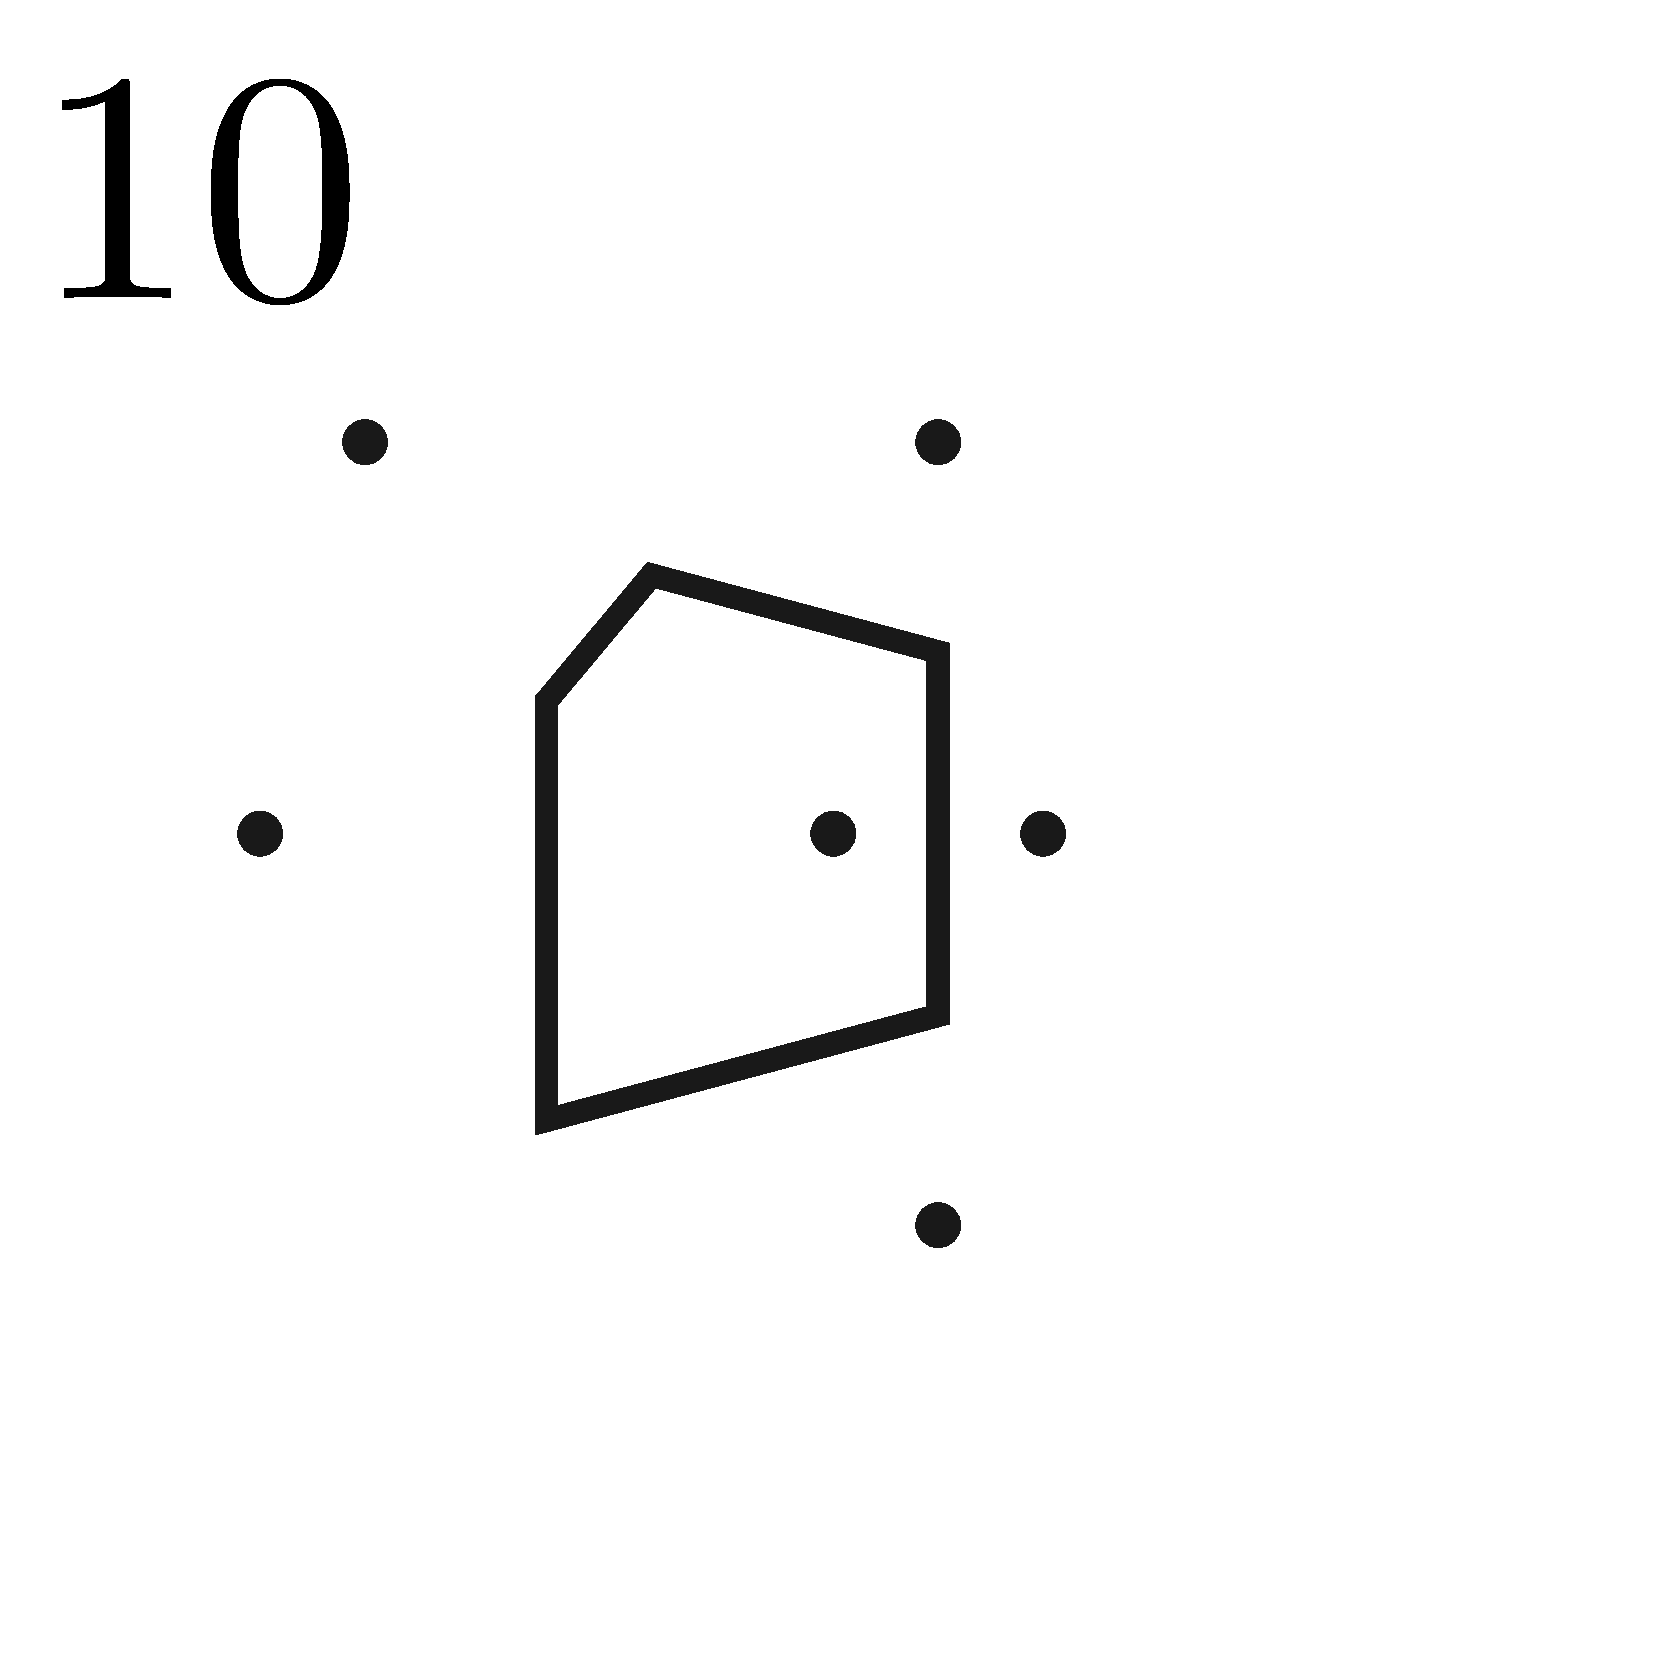
\includegraphics[width=0.14\textwidth]{finiteSectionForTileGeneration/tile010}
\caption{First line are the polygons from the Figure \ref{fig:finiteSectionForTileGeneration:more} and the second line are the slightly larger ones that also appear in the quasicrystal.}
\label{fig:finiteSectionForTileGeneration:bigger}
\end{figure}

The intersection is a superset of the section. The Figure \ref{fig:intersectionsComparison} shows the intersections for first polygons of each line in the Figure \ref{fig:finiteSectionForTileGeneration:bigger}.

\begin{figure}[h]
\centering
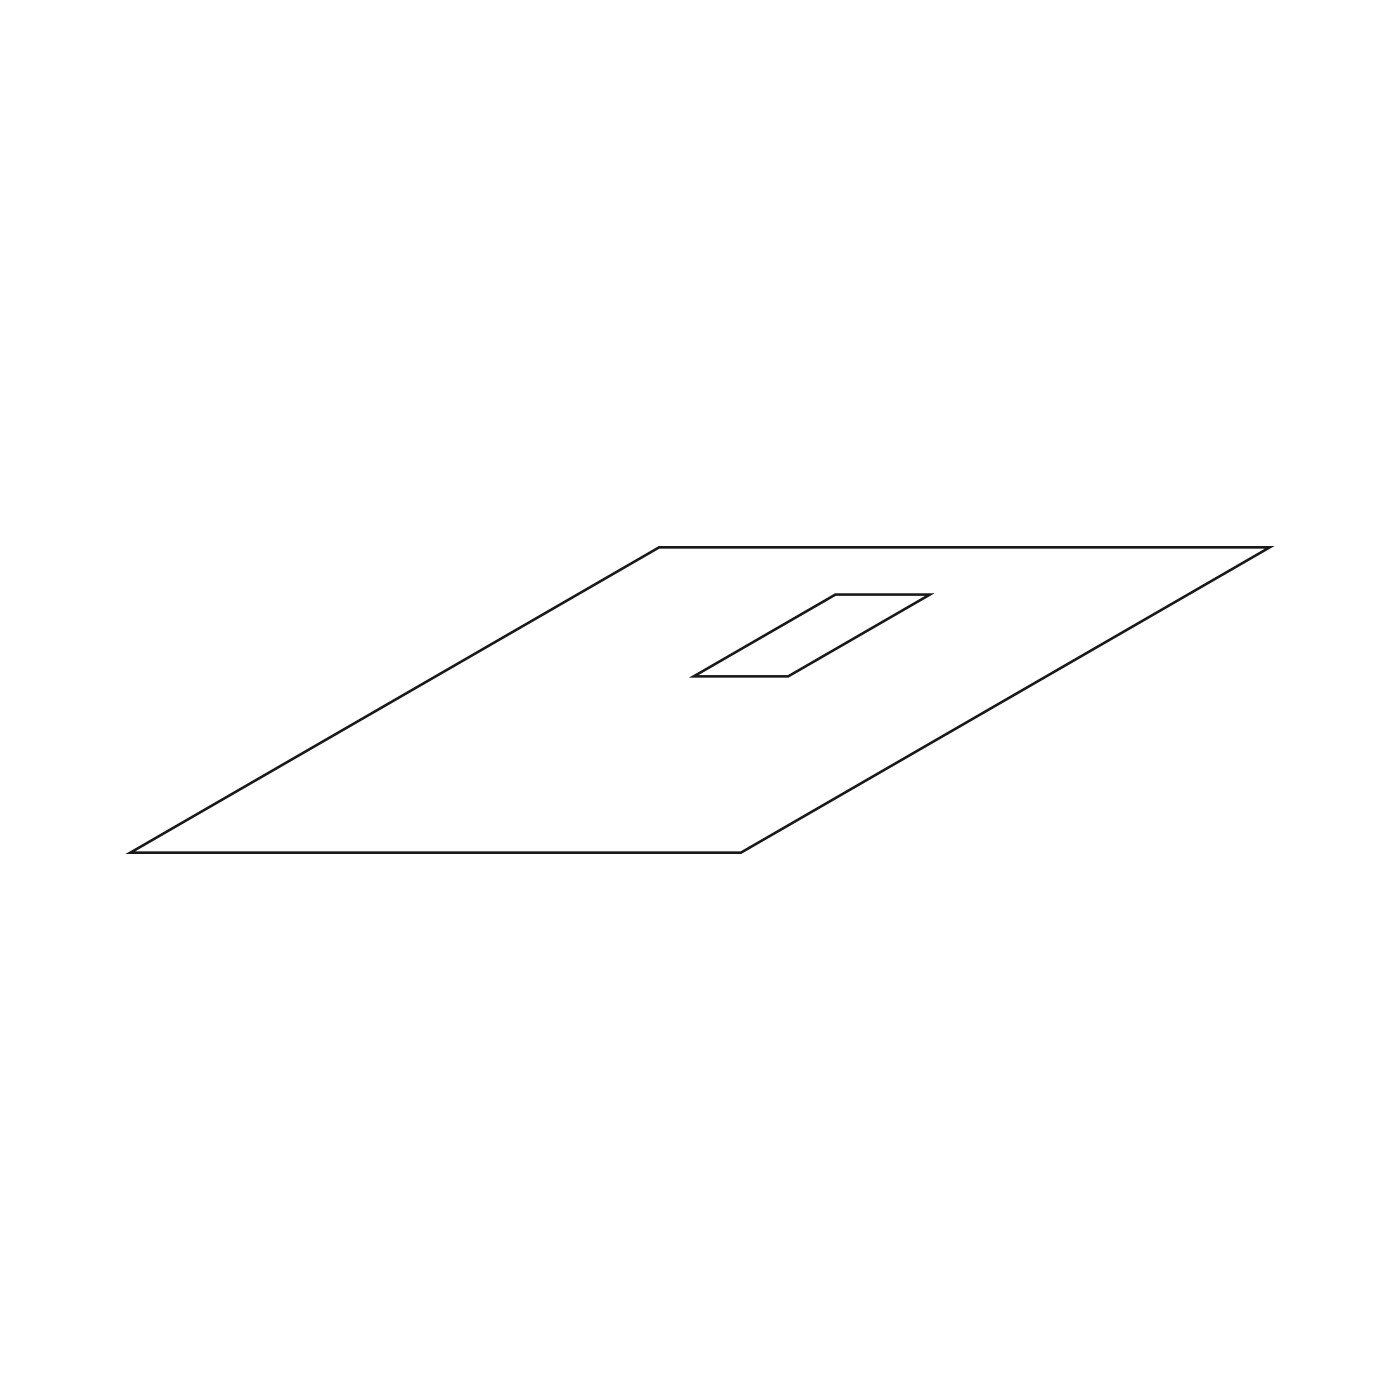
\includegraphics[width=0.4\textwidth]{catalogRhombusSingle/tile003_window}
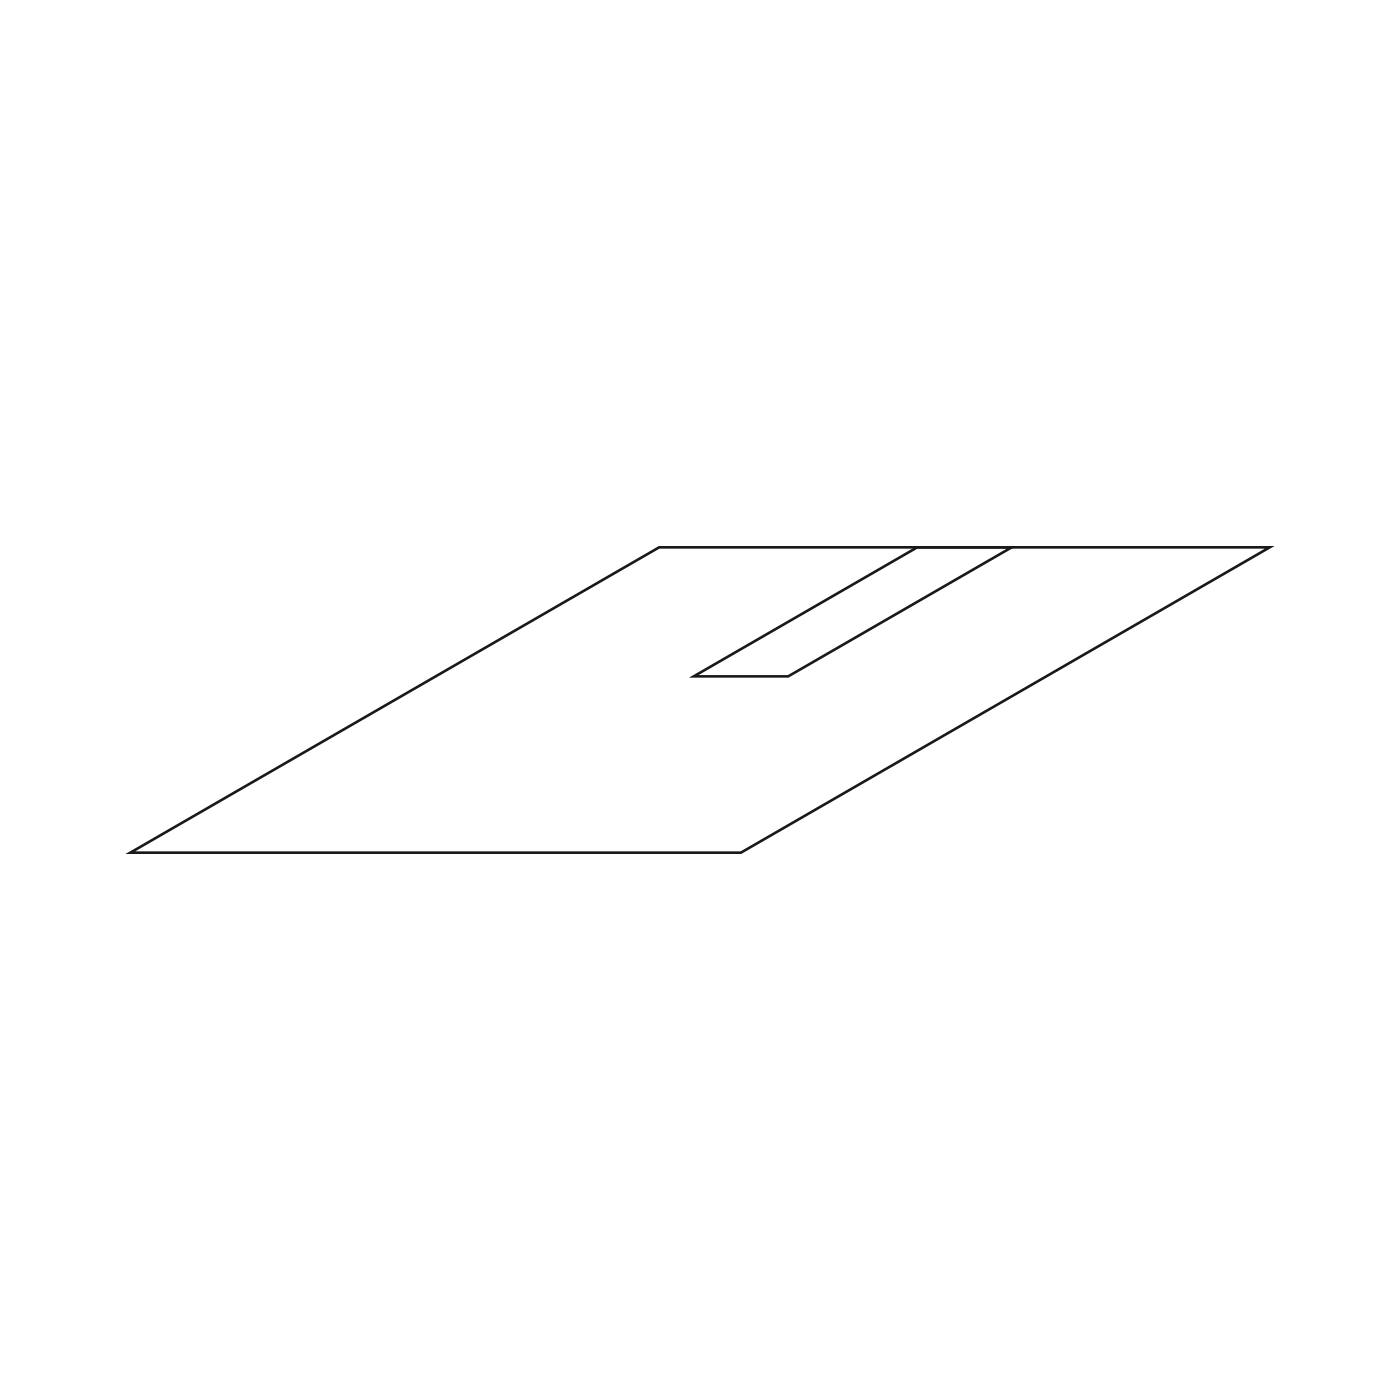
\includegraphics[width=0.4\textwidth]{catalogRhombusSingle/tile007_window}
\caption{Intersections for first polygons in each line in the Figure \ref{fig:finiteSectionForTileGeneration:bigger}.}
\label{fig:intersectionsComparison}
\end{figure}

Clearly the first intersection is a subset of the second one and also the corresponding polygons are in the same relation. Therefore a conclusion can be drawn that if the $\ast$ image falls within the smaller intersection, it's polygon will be the smaller one because the domain of the smaller polygon will by present in the quasicrystal. Only if the $\ast$ image of the center fall outside the smaller intersection but inside the larger one will it's polygon be the larger one (Figure \ref{fig:intersectionOverlap}).

\begin{figure}[h]
\centering
\includegraphics[width=0.16\textwidth]{catalogRhombusSingle/tile003}
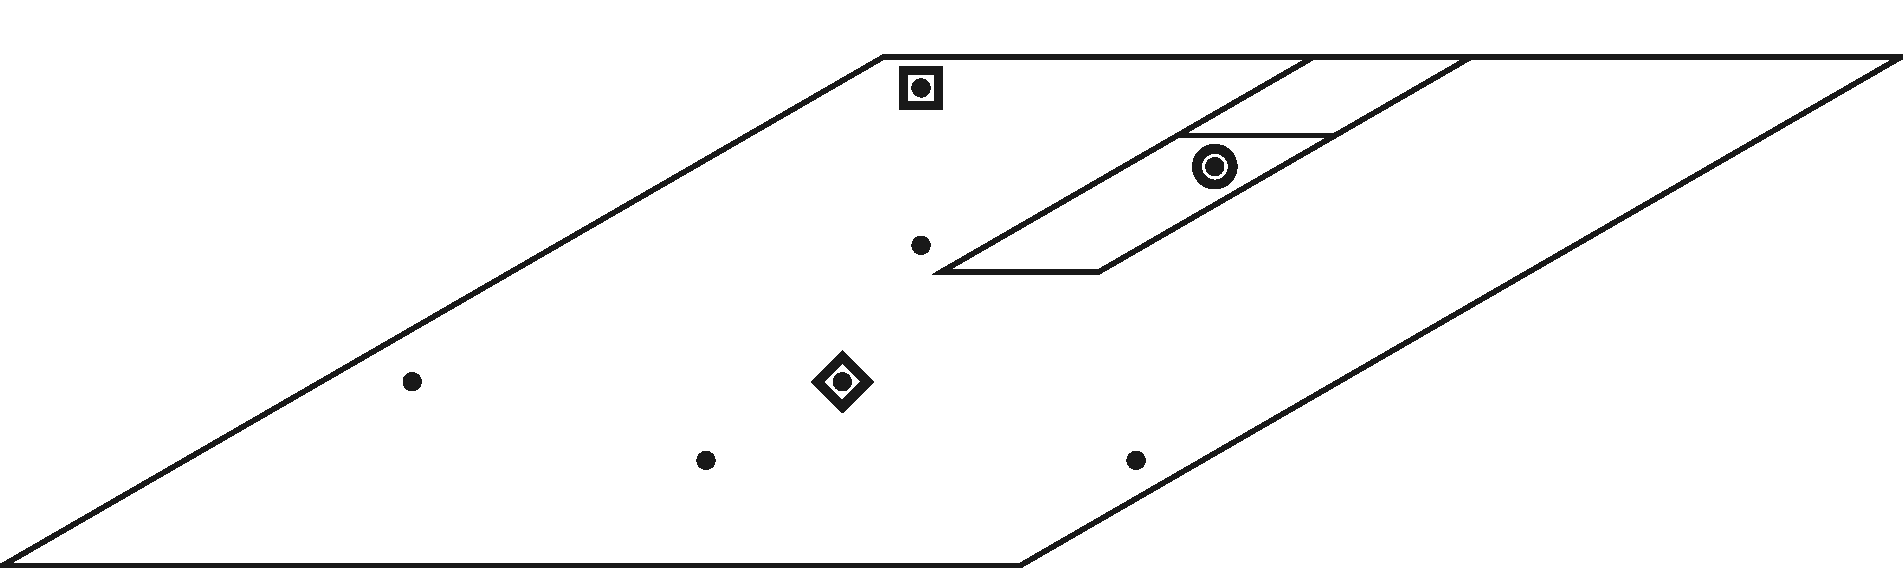
\includegraphics[width=0.4\textwidth]{catalogRhombusSingle/tile003_windowSectionInside}
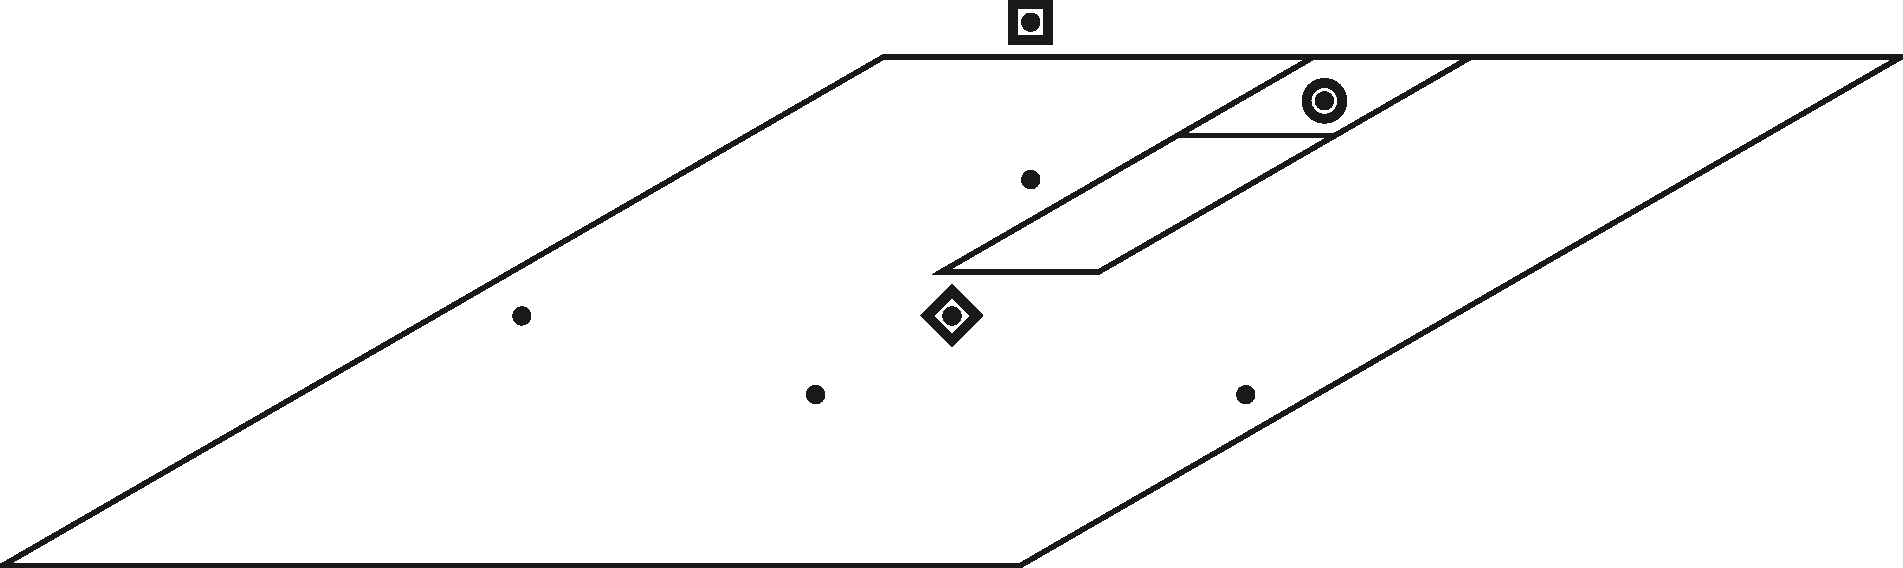
\includegraphics[width=0.4\textwidth]{catalogRhombusSingle/tile003_windowSectionOutside}
\caption{The points in the left window correspond to the smaller polygon, the {\scriptsize $\Diamond$} marked point is not a member of the domain. The points in the right window correspond to the larger polygon, the {\scriptsize $\square$} marked point no longer fit inside the window and so the {\scriptsize $\Diamond$} marked point becomes a member of the domain.}
\label{fig:intersectionOverlap}
\end{figure}

Similar situation happens with the polygons in the Figure \ref{fig:morePolygonsExample}.

\begin{figure}[h]
\centering
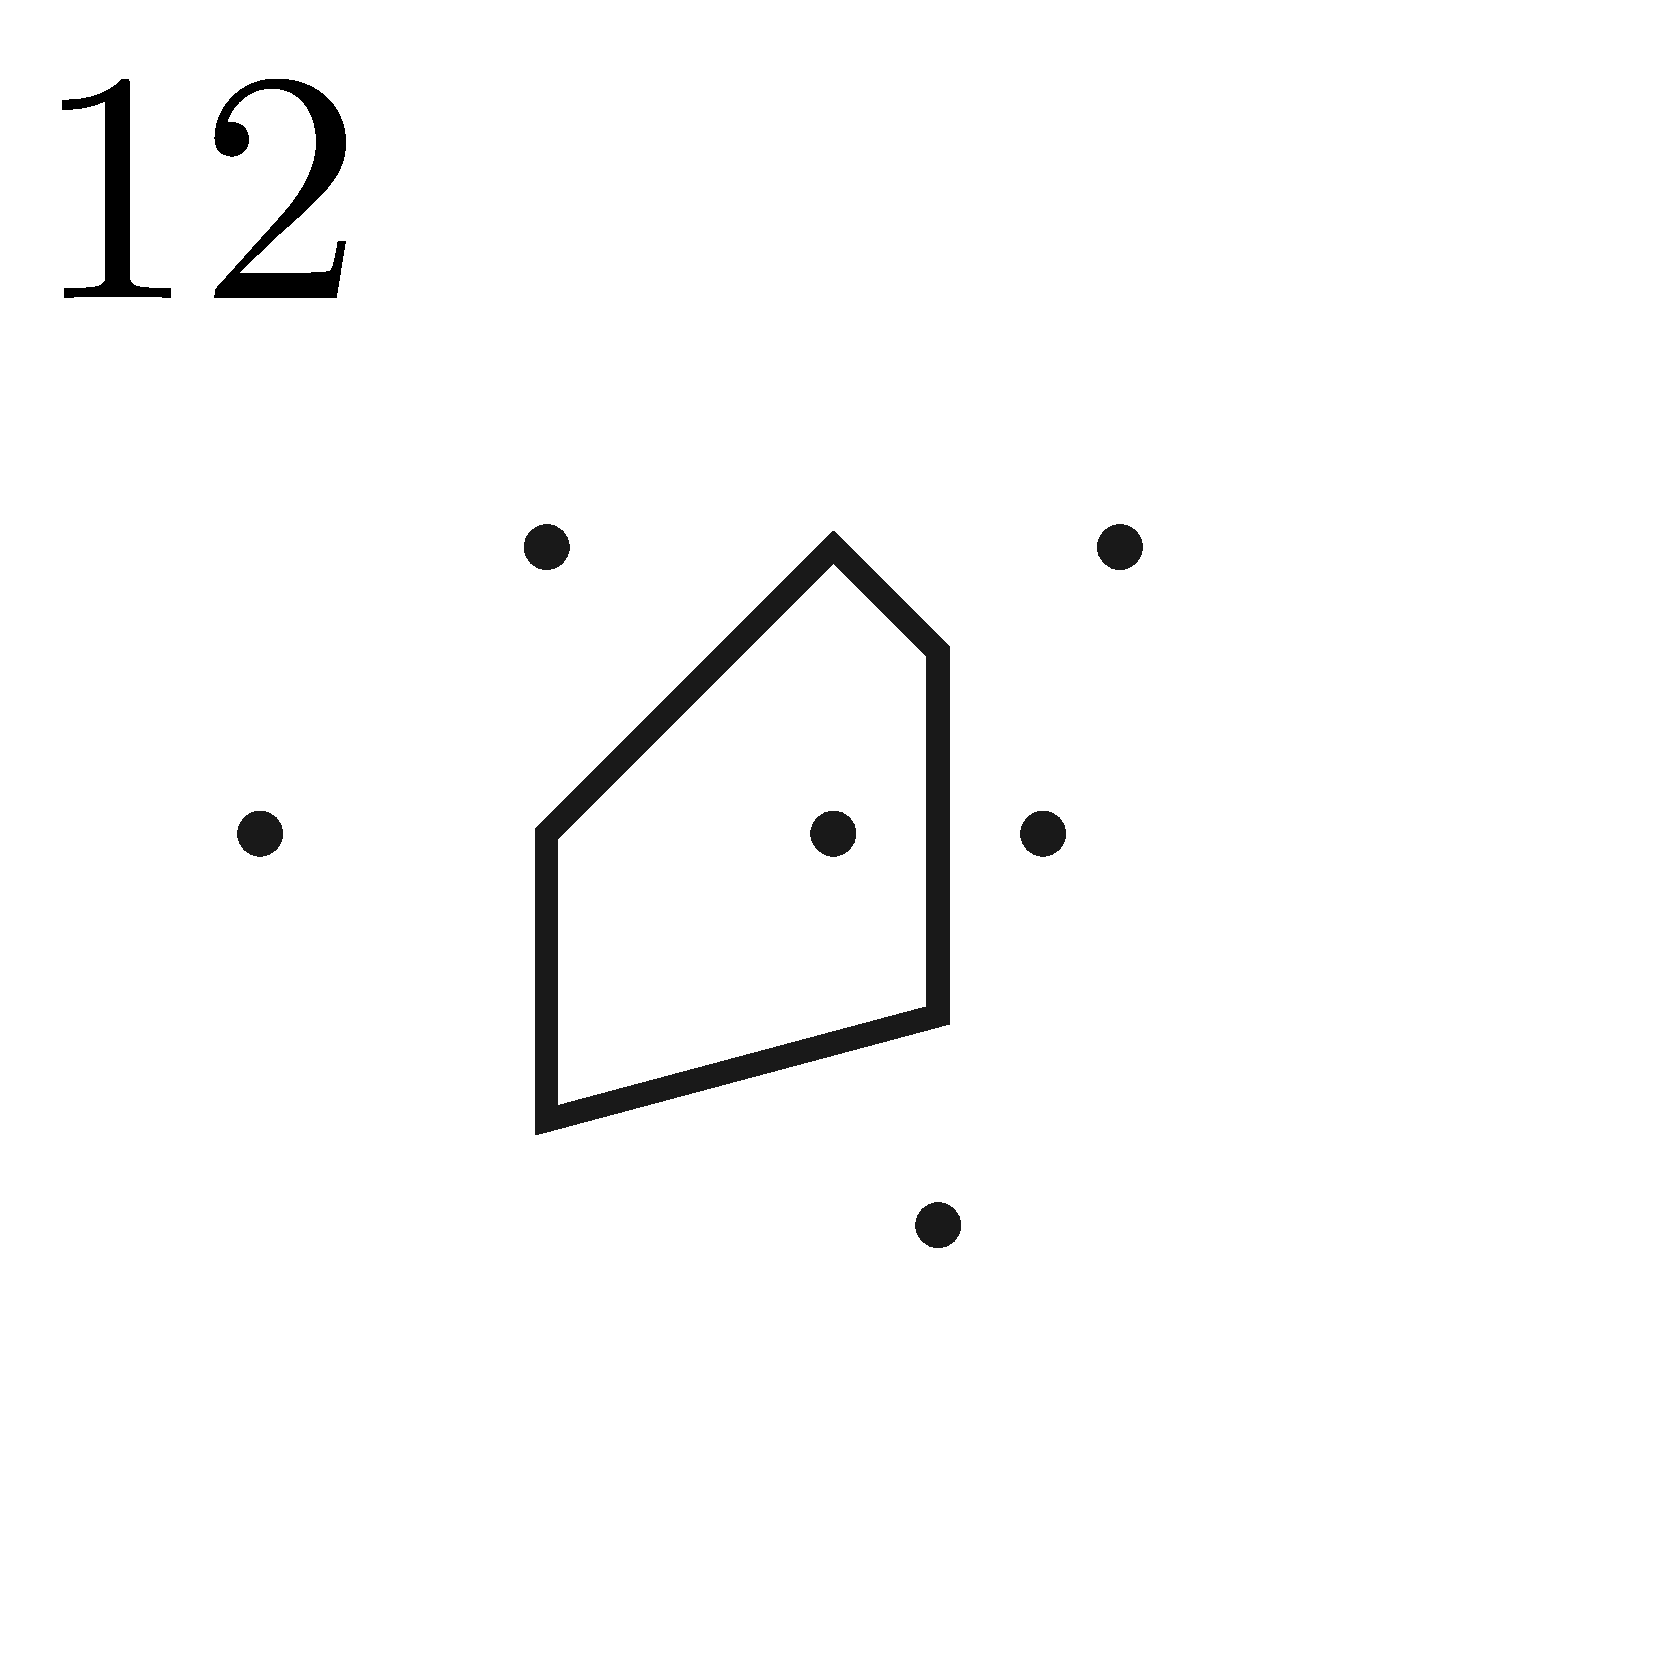
\includegraphics[width=0.24\textwidth]{catalogRhombusSingle/tile012}
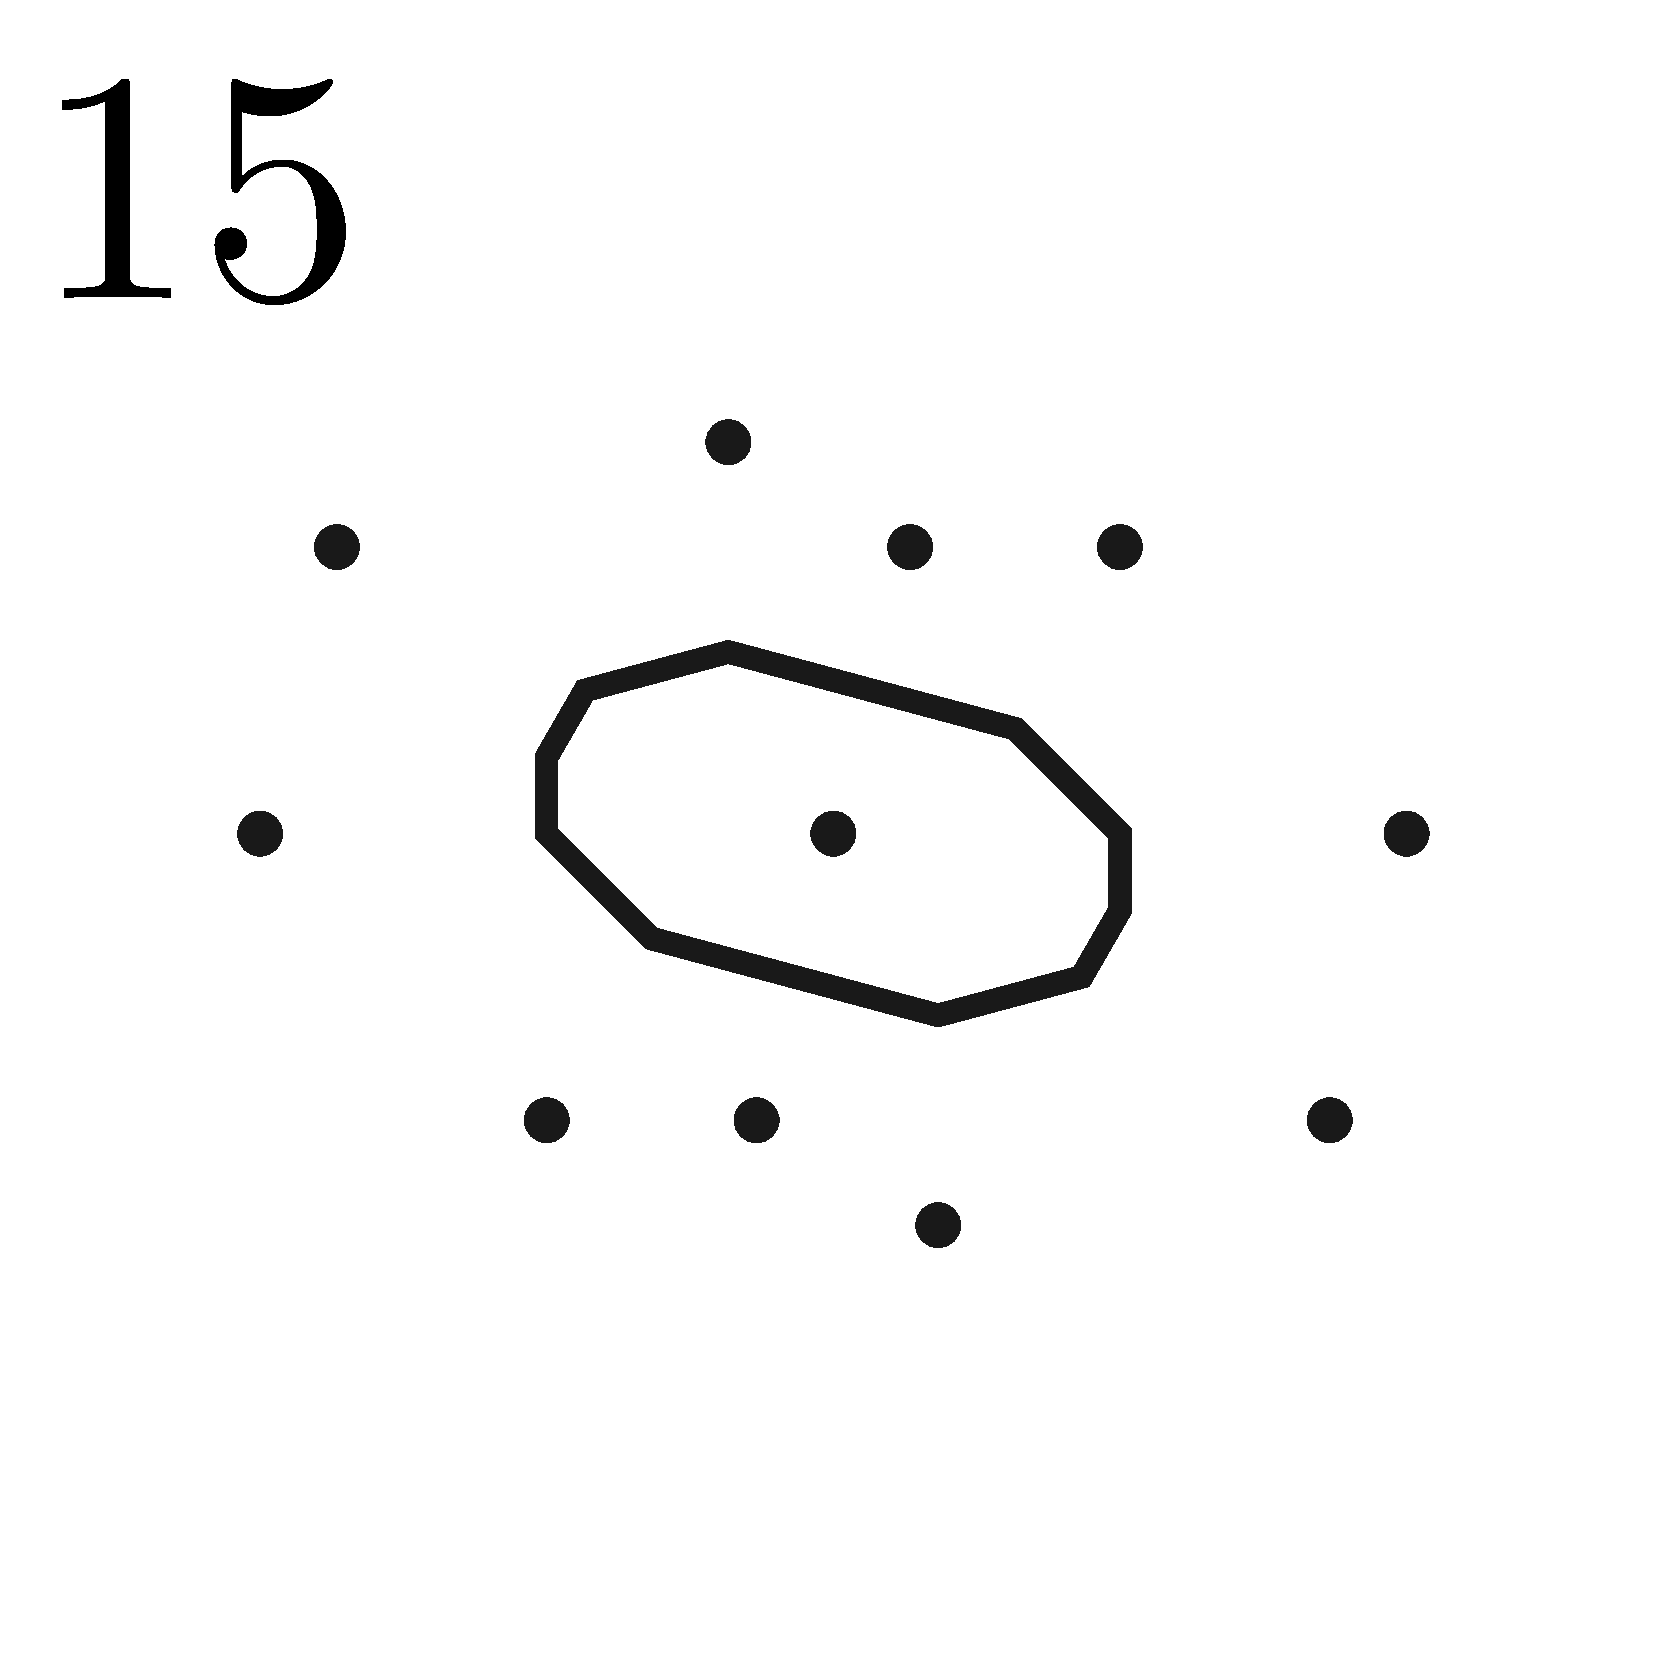
\includegraphics[width=0.24\textwidth]{catalogRhombusSingle/tile015}
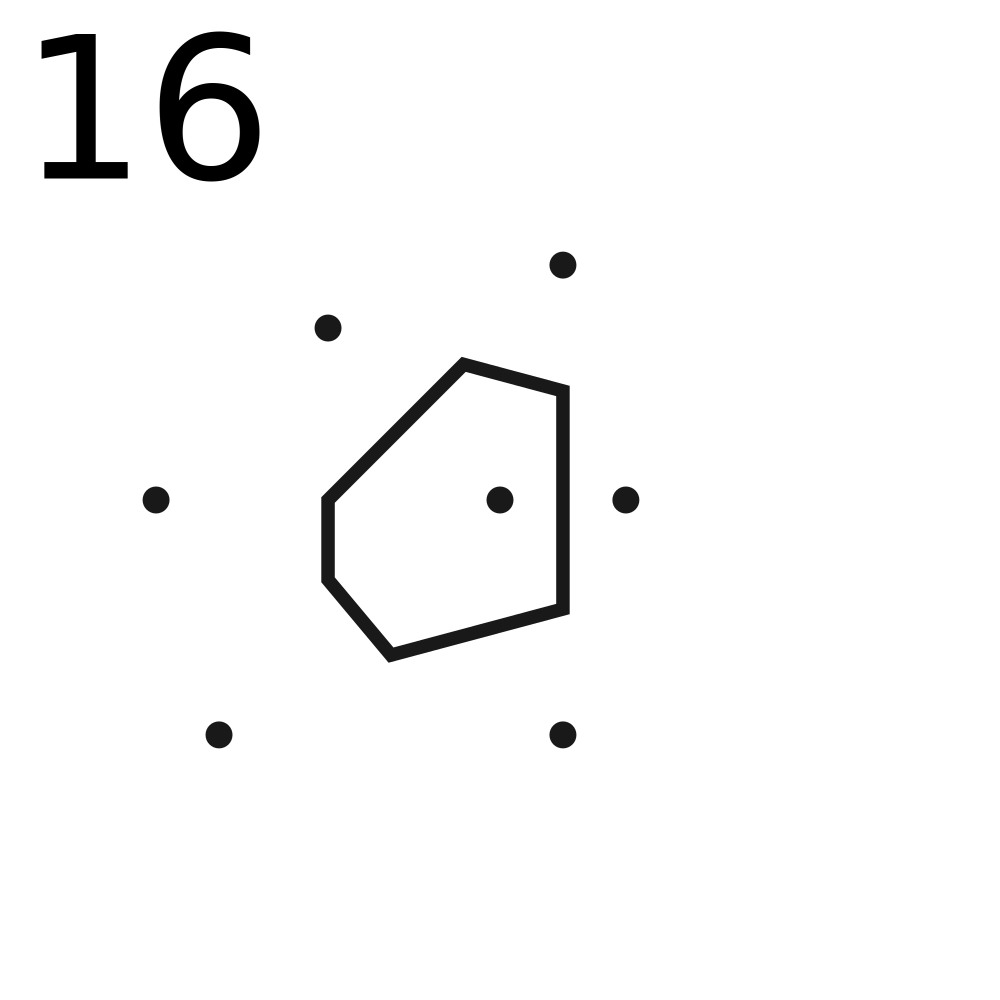
\includegraphics[width=0.24\textwidth]{catalogRhombusSingle/tile016}
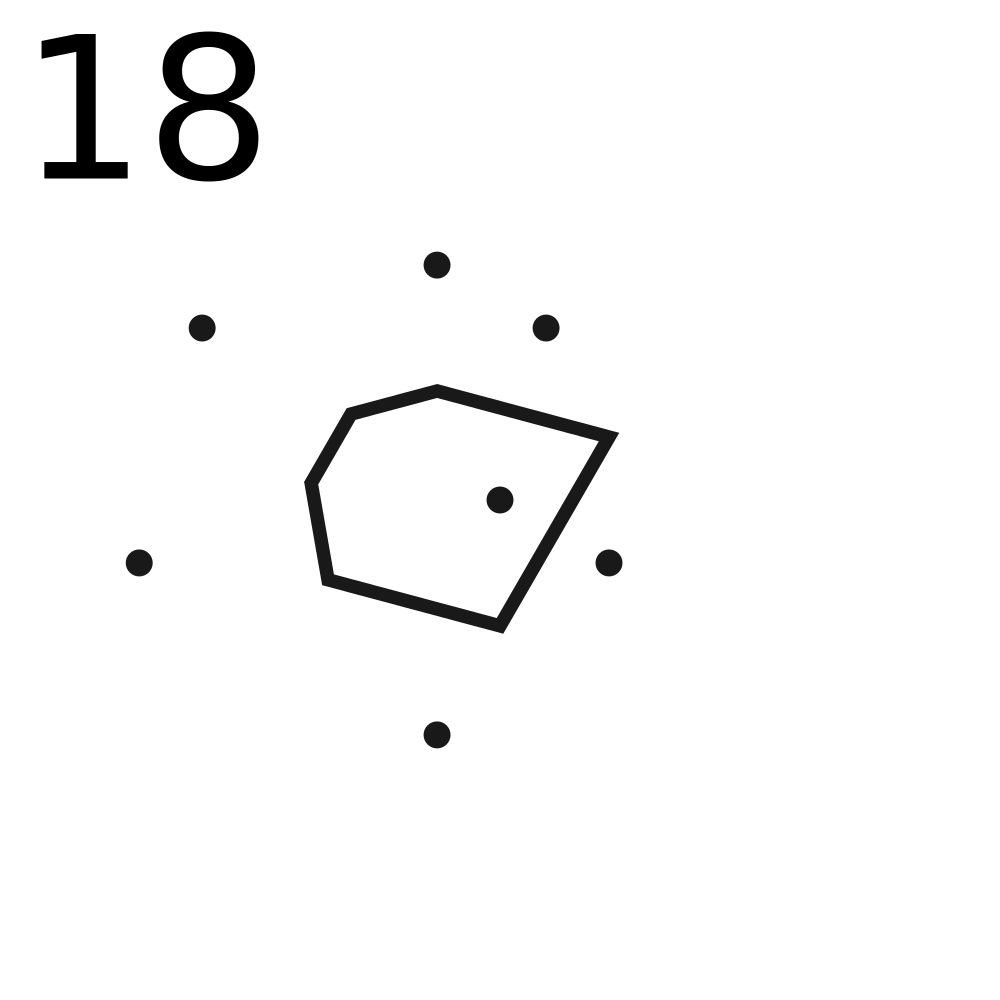
\includegraphics[width=0.24\textwidth]{catalogRhombusSingle/tile018}
\caption{These voronoi polygons also have overlapping intersections.}
\label{fig:morePolygonsExample}
\end{figure}

\paragraph{Summary}
This section covered the algorithms for generating all different shapes of voronoi polygons for a single rhobic window and for dividing said window into sections by the different shapes. Next section will achieve the same for all rhombic window sizes.

\end{document}
